%! Author = joeda
%! Date = 2022-12-19

% Preamble
\documentclass[11pt]{article}
%\linespread{2} %double interligne
\usepackage{geometry}
\geometry{margin=1in}
% Packages
\usepackage{amsmath}
\usepackage{graphicx}
\usepackage{caption}
\usepackage{subcaption}
\usepackage{subfigure}
\usepackage{biblatex}
%\usepackage[backend=biber]{biblatex}

\usepackage{blindtext}%section management
\usepackage{xcolor} %color management

\newcommand\myworries[1]{\textcolor{red}{#1}}

\usepackage[utf8]{inputenc} % Pour les accents
\usepackage[english]{babel}  % Language hyphenation and typographical rules
\usepackage{csquotes}
\usepackage{hyperref}
\usepackage{amsfonts}

\usepackage{float} % for figure placement
\usepackage{booktabs} %for table

\usepackage{multicol} % for multi-column itemize


\addbibresource[backend=biber]{reference.bib}
% Document
\begin{document}


    \section{Introduction}

    \subsection{CheXnet}

        Our project is based on the recent development by a Stanford team on the CheXnet~\cite{chexnet}
        and CheXpert~\cite{chexpert} project. These two projects had  one common goal : to develop an AI
        able to help, or in time maybe even replace radiologists for the analysis of Chest X-Ray (CXR) images. Their
        first project , CheXnet, was based on a deep learning model that was able to predict 14 different diseases
        from a CXR image.
        While they did manage some interesting results, many criticism arose from the medical community. One such
        critic, the Dr. Lauren Oakden-Rayner, a radiologist and a Senior Research Fellow at the Australian Institute
        for Machine Learning, did a deep dive into the project, going as far as having a back and forth with the
        author to help them publish edited version of their paper. As these criticism were quite interesting and led
        to the follow-up project, we will go over them in the next section.


    \subsection{Criticism}
        Dr. Oakden-Rayner did a deep dive into the project, and before going into the CheXpert project, did a good
        recapitulative of the issues with the CheXnet project~\cite{chexpert_critic}. In her own word :
        \begin{quote}
            \begin{enumerate}

                \item Variability: Lots of very similar cases, because there were many patients who had numerous studies (i.e.,
                repeat ICU films). For example, while only 7\% of patients had more than 10 films, this still made up 45\% of the
                        total dataset. This means that while the overall number of films in the dataset is impressive, the variability is equivalent to a much smaller dataset (we might call this the effective size of the dataset).
                \item Labelling method: Labelled via natural language processing, which both has an error rate as a method, and an
                        irreducible error due to the fact that reports don’t actually describe images very thoroughly.
                \item Labelling quality: Labels didn’t seem to match images very well, on the order of 30-90\% error
                rates for the various classes.
                \item Label structure: Some of the labels were very difficult to interpret, with a range of labels that
                describe pretty much the same visual appearances (like “consolidation”, “pneumonia”, “infiltration”).
                \item Hidden stratification: Some of the labels contained clinically important subgroups (strata) that
                were not labelled, for example the pneumothorax (collapsed lung) class didn’t distinguish between deadly untreated pneumothoraces and completely safe, well-treated pneumothoraces. These subsets seemed to lead to models that learned useless and potentially dangerous things, like only identifying treated pneumothoraces and missing untreated ones.
                \item Documentation: The CXR14 paper, and the additional documentation (here), do not adequately
                describe the data. It is unclear how the labels were defined, what the cohort characteristics are, or how the dataset could reliably be used.
                \item Image quality: The images in the dataset have been downsampled (from 3000 x 2000 pixels to 1024 x
                1024) as well as having heavily reduced the number of grey-levels (normally between 3 and 4 thousand, now only 255). This severely harms interpretation of many conditions. Of note, subtle pneumothoraces, small nodules, and retrocardiac opacities become nearly impossible to diagnose for a human expert.
            \end{enumerate}
        \end{quote}
        The full detail of the criticism can be found in the blog post~\cite{chexnet_critic}.

    \subsection{CheXpert}


        The second project, CheXpert, was based on the same model but with a larger dataset and a more precise analysis
        of the diseases. While they kept the 14 original diseases, they mainly focus on 5 different diseases from a CXR image
        (Atelectasis,Cardiomegaly, Consolidation,Edema and Pleural Effusion). It corrected a few of the criticsm
        from the last project, and had a different goal. While the Stanford team focused on building the deep learning model
        for the CheXnet project, which used publicly available data from the National Institute of Health (NIH),
        which was criticised for being often mislabeled, this project focused on building a new dataset. They gathered
        over 400 000 images from the Stanford hospital for the project, and while most label were derived from an
        automated labeler (to convert the text annotation of the radiologists in the patient's file), which assigned
        a positive, negative , or uncertain flag to each of the label for a given report. The validation
        and test dataset reviewed by a panel of three radiologists to ensure the quality of the dataset.
        This is a necessary steps as the evaluation of CXR images is a very
        complex task, with not always a clear answer. In their CheXnet project, they evaluated the performance of
        their radiologists to be at around 0.4 with the F1-score. This is a rather low score, and therefore explains
        the need to have a validation/test set reviewed by a panel of radiologists.

        While most of the dataset was released, they kept the test set private to evaluate the performance of models
        submitted to them for the CheXpert competition they created. This competition was launched in 2019 and is still
        ongoing. At the moment of writing this report, the best model has an AUC of 0.93, a score achieved by both
        the Big Data Institute\cite{hierarchical} and the Deep AUC maximization model~\cite{DeepAUC}, which is a
        very impressive score.


    \subsection{Our project}

        For our project, while we mostly worked with the CheXpert dataset, we also started building our own, using
        data from the different hospitals covered by the CIUSSS Centre-Sud-de-l'Île-de-Montréal (CCSMTL)
    \myworries{Cite?}. Sadly delays in the acquisition of the data and the lack of a clear protocol for the
    processing of it meant that we were only able to start working on it by September.

    we also had to deal with the fact that this data was not labelised yet. We received the image in the DICOM
    format\myworries{cite} and had to convert them to a more usable format (jpeg). The images were linked with a text
    report from the radiologist, which we had to convert to a label. Since our text were in french, and that most
    ressources available were in english, we had to develop our own rule-based system to convert the text to a label.
    This part of the project was done by another student, Maxime Fournier, and will therefore not be discussed in
    details here. \myworries{Add in appendix?}

    Once the data was ready, we separated the dataset into a training, validation and test set, with 300 patients per
    classes in the validation set, and 300 (20 images per classes) in the test set.
    We ensured there were no patient leakage between the different sets(a patient seen during training should not
    have images present within the test or validations set), and we also sampled the images such that to ensure a
    good representation of the different diseases in the dataset.

    Sadly, the CCSMTL was not able to provide us with expertise in the form of radiologists to review the dataset, or
    our conversion from text to label. We therefore had to rely solely on our interpretation of the text and the
    opinion given by the one radiologist who initially reviewed the images. This is a major limitation of our dataset,
    and might explain the poor performance of our model later on. At the moment of writting\footnote{2023-01-03}, we
    were still waiting  for the CCSMTL to provide us with a second meeting with the radiologists, in order to
    hopefully secure time to have them review and validate our test dataset \footnote{While it would be very
    important to also have a validation dataset validated by radiologist, the CCSMTL was reluctant to try and provide
    us with the ressources to do so.} . Please also note that most
    of our analysis will be conducted on the CheXpert dataset, both as it has been validated by radiologists, and
    since the data from the CCSMTL was not yet ready yet \footnote{The data was only fully delivered to us towards
    the end of the internship}.


    \section{Data Analysis}

    The first step of any ML project is to analyse the data available to us. Let's start with the CheXpert dataset.
    We will first look at the distribution of the classes. As we can see
    in~\ref{fig:histogram_chexpert_train}, the dataset is not balanced. We will need to take this into account when
    training our model. We also can see that the three least represented classes are under 10 000 images, which might
    make it difficult to train a model that can accurately predict them. A good use of data augmentation techniques
    will probably be necessary to train a model that can accurately predict these classes.

    Now looking at the distribution of the classes in the validation set, we can see that the classes are more evenly
    split. This is a good sign, as it means that the validation set will be a good representation of the performance
    on the different classes. This is however not true for all classes, as Fracture has no images at all present in
    the validation dataset. Four other classes also have less than 10 images present, which will make it difficult to
    know for sure whether the model is able to predict them accurately. The results for those classes will most
    likely need to be ignored.

    For the CCSMTL dataset, we can see in the training dataset~\ref{fig:histogram_ciusss_train} that we have an even stronger imbalance than in the
    CheXpert dataset. Images without any disease constitues almost 25\% of the dataset, with over 100 000 images
    while some classes have less that 5000 images. We will have to correct for this while training, with strategies
    such as weighting the loss, data augmentations and undersampling the classes with too many images.

    In the validation dataset~\ref{fig:histogram_ciusss_train}, we did not simply randomly sampled the images, we can
    see the distribution of images differs from the training dataset. However, an imbalance is still present, as some
    disease might require more images than others to be accurately predicted or treated. However, we can see that we
    still have a minimum of 300 images per classes, which should be enough to evaluate the performance of the model.
    We should however stay weary of this imbalance, since if we simply used a loss (such as the cross entropy), to
    see the performance of our model, the overrepresented classes might also be overrepresented in the loss, and thus
    bias our choice of hyperparameters. To correct for this, we can use metrics that takes into account the imbalance
    present in our dataset, such as the F1-score, or the AUC.~\cite{metrics}.
\newpage
    \begin{figure}[h!]
         \centering
         \begin{subfigure}[b]{0.48\linewidth}
             \centering
             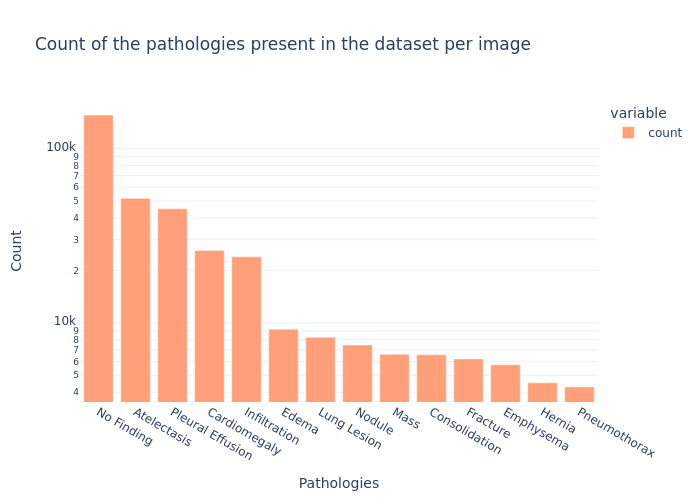
\includegraphics[width=\linewidth]{plots/histogram_ciusss_train}
             \caption{CIUSSS's training dataset}
             \vspace{4ex}
             \label{fig:histogram_ciusss_train}
         \end{subfigure}
         \hfill
         \begin{subfigure}[b]{0.48\linewidth}
             \centering
             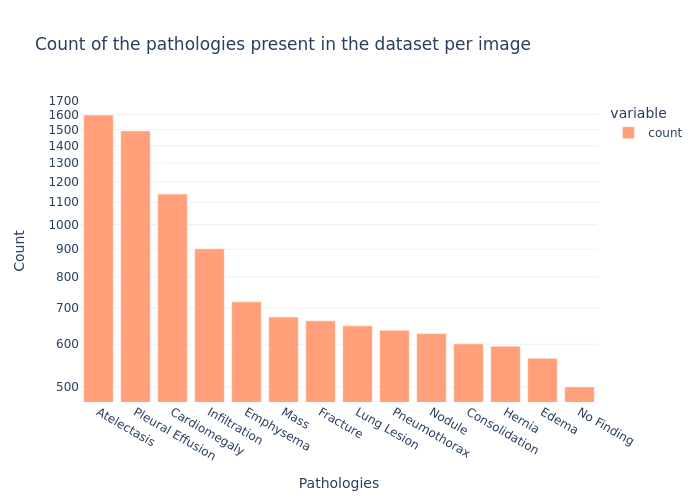
\includegraphics[width=\linewidth]{plots/histogram_ciusss_valid}
             \caption{CIUSSS's validation dataset}
             \vspace{4ex}
             \label{fig:histogram_ciusss_valid}
         \end{subfigure}


         \begin{subfigure}[b]{0.48\linewidth}
             \centering
             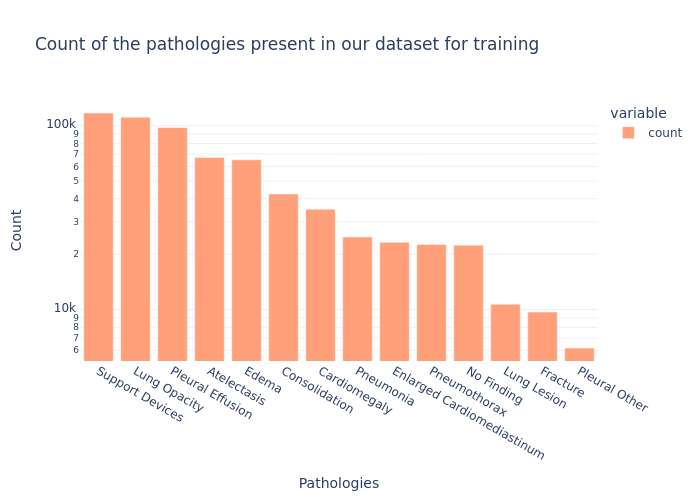
\includegraphics[width=\linewidth]{plots/histogram_chexpert_train}
             \caption{CheXpert's training dataset}
             \vspace{4ex}
             \label{fig:histogram_chexpert_train}
         \end{subfigure}
         \hfill
         \begin{subfigure}[b]{0.48\linewidth}
             \centering
             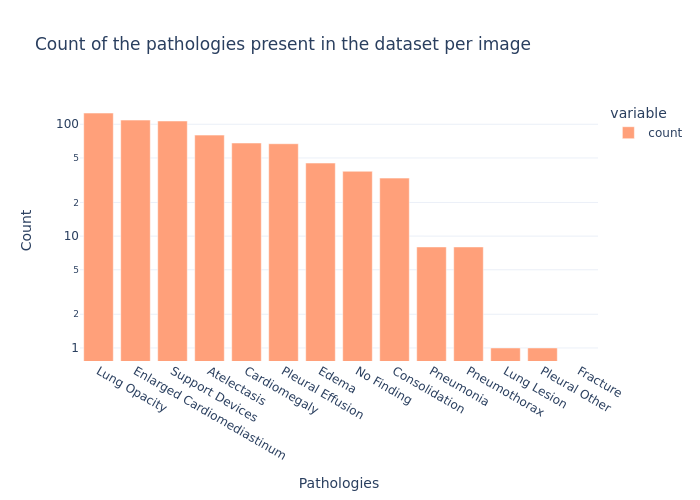
\includegraphics[width=\linewidth]{plots/histogram_chexpert_valid}
             \caption{CheXpert's validation dataset}
             \vspace{4ex}
             \label{fig:histogram_chexpert_valid}
         \end{subfigure}

         \caption{Histogram for the different labels present in the CIUSSS and CheXpert dataset}
         \label{fig:histogram_classes}
    \end{figure}
\newpage


    Another important thing to look at could be the correlation between diseases, to identify potential biases in the
    data. To account for uncertainty labels, we will simply replace the uncertainty labels by a positive label for
    this analysis.

    Looking at the Chexpert's correlation graph (see~\ref{fig:chords_chexpert_train} and~\ref{fig:chords_chexpert_valid}),
    we can see that the correlation between diseases is quite high. This is slightly worrying, as it means that the data could be biased
    towards a specific disease. We can also see that the correlation is higher in the validation dataset than in the training
    dataset. This is expected, as the validation dataset is smaller and therefore more likely to have a higher correlation
    between diseases.


    However, when we look at the CIUSSS's correlation graph (see~\ref{fig:chords_ciusss_train} and~\ref{fig:chords_ciusss_valid}), we observe a way lower correlation level between pathologies.
    It might also be due to a difference in the population but this explanation does not seem quite likely

    Assuming the preponderance of diseases is the same between the population visiting the Stanford's hospital and
    the CIUSSS CCSMTL, we are left to assume that the quality of the data is different from the Stanford dataset. Whether it is better or worst is to verify.


\newpage
\begin{figure}[h!]
     \centering
     \begin{subfigure}[b]{0.45\linewidth}
         \centering
         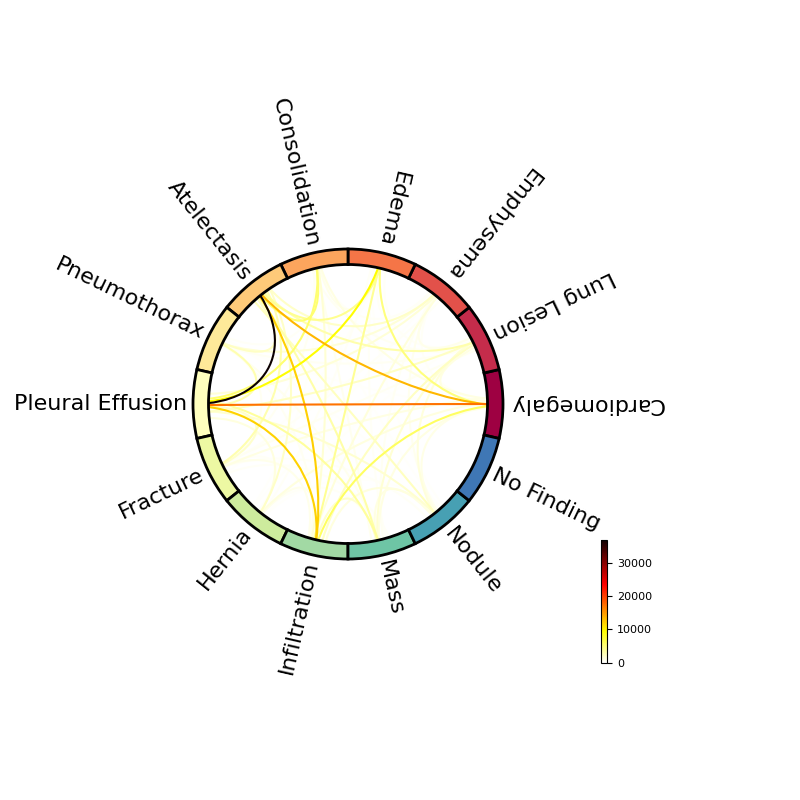
\includegraphics[width=\linewidth]{plots/chords_ciusss_train}
         \caption{CIUSSS's training dataset}
         \vspace{4ex}
         \label{fig:chords_ciusss_train}
     \end{subfigure}
     \hfill
     \begin{subfigure}[b]{0.45\linewidth}
         \centering
         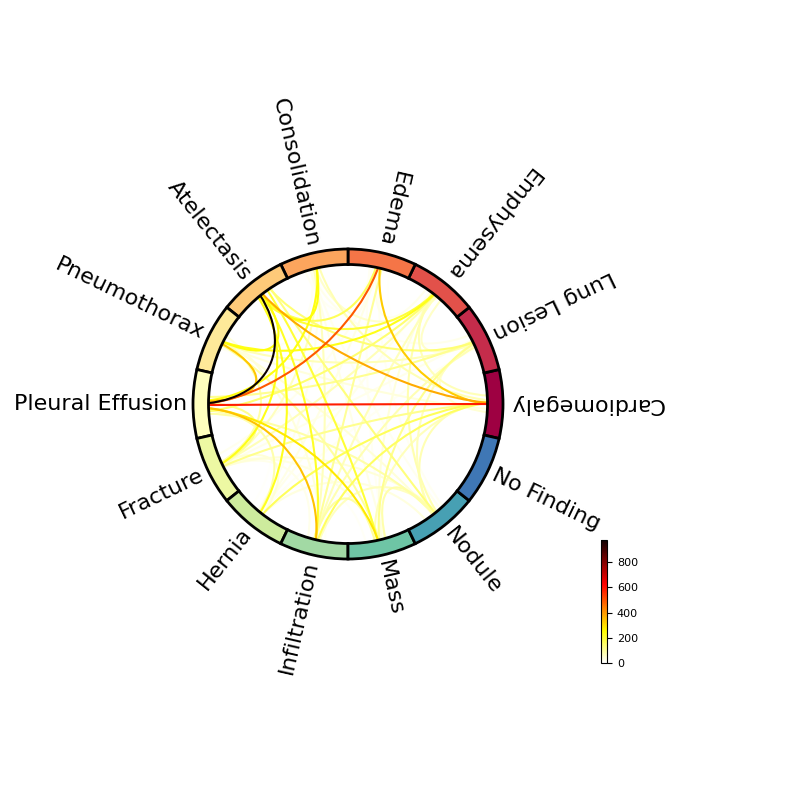
\includegraphics[width=\linewidth]{plots/chords_ciusss_valid}
         \caption{CIUSSS's validation dataset}
         \vspace{4ex}
         \label{fig:chords_ciusss_valid}
     \end{subfigure}


     \begin{subfigure}[b]{0.45\linewidth}
         \centering
         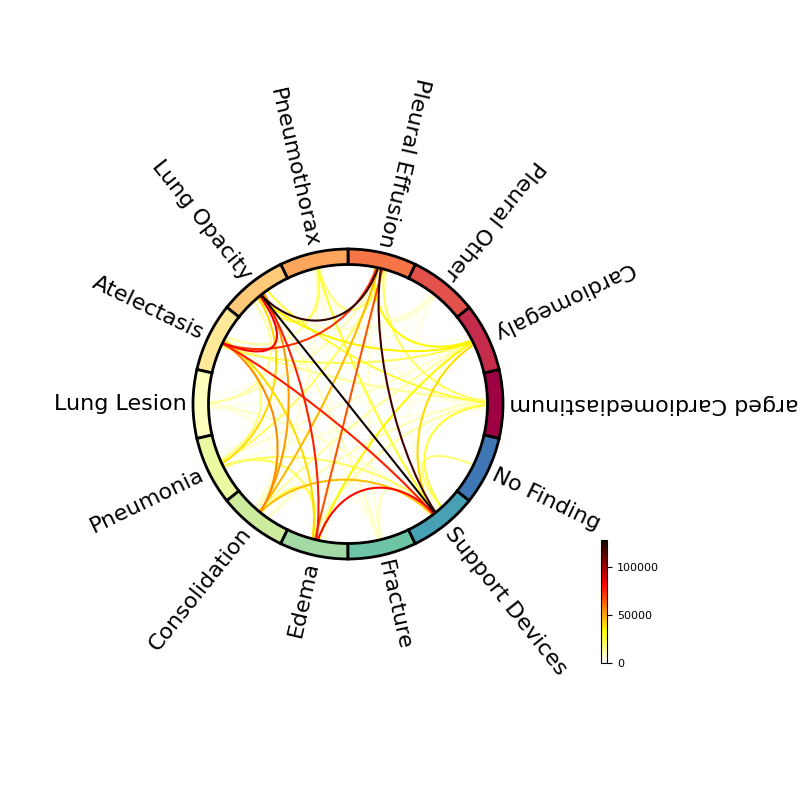
\includegraphics[width=\linewidth]{plots/chords_chexpert_train}
         \caption{CheXpert's training dataset}
         \vspace{4ex}
         \label{fig:chords_chexpert_train}
     \end{subfigure}
     \hfill
     \begin{subfigure}[b]{0.45\linewidth}
         \centering
         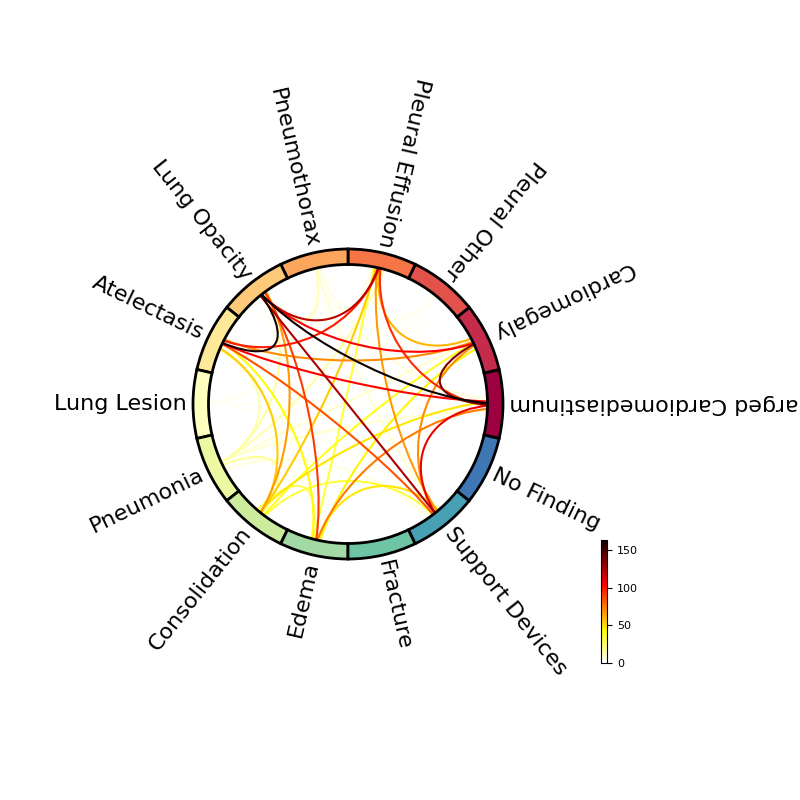
\includegraphics[width=\linewidth]{plots/chords_chexpert_valid}
         \caption{CheXpert's validation dataset}
         \vspace{4ex}
         \label{fig:chords_chexpert_valid}
     \end{subfigure}

     \caption{Histogram for the different labels present in the CIUSSS and CheXpert dataset}

\end{figure}
\newpage
\begin{figure}[H]
     \centering
     \begin{subfigure}[b]{0.45\linewidth}
         \centering
         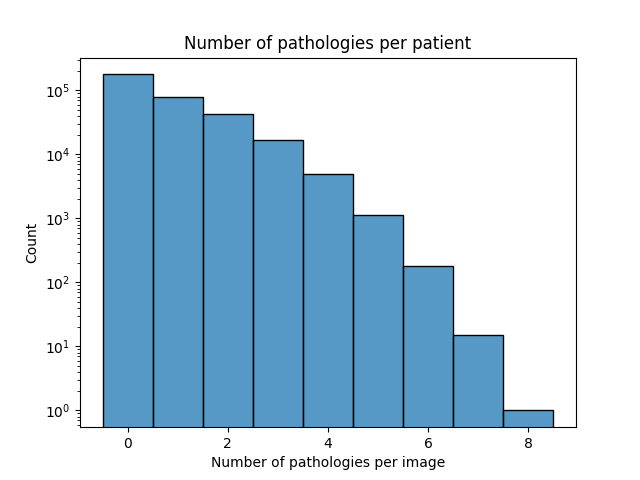
\includegraphics[width=\linewidth]{plots/disease_count_ciusss_train}
         \caption{CIUSSS's training dataset}
         \vspace{4ex}
         \label{fig:count_ciusss_train}
     \end{subfigure}
     \hfill
     \begin{subfigure}[b]{0.45\linewidth}
         \centering
         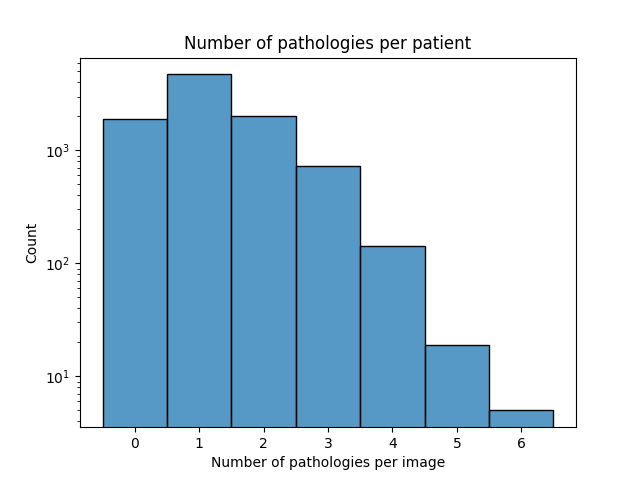
\includegraphics[width=\linewidth]{plots/disease_count_ciusss_valid}
         \caption{CIUSSS's validation dataset}
         \vspace{4ex}
         \label{fig:count_ciusss_valid}
     \end{subfigure}


     \begin{subfigure}[b]{0.45\linewidth}
         \centering
         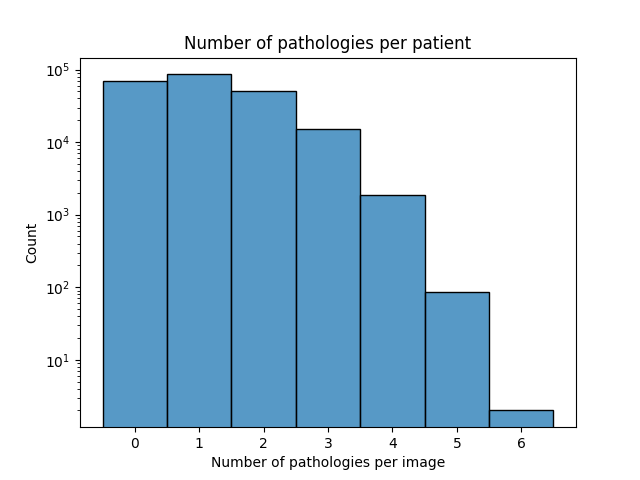
\includegraphics[width=\linewidth]{plots/disease_count_chexpert_train}
         \caption{CheXpert's training dataset}
         \vspace{4ex}
         \label{fig:count_chexpert_train}
     \end{subfigure}
     \hfill
     \begin{subfigure}[b]{0.45\linewidth}
         \centering
         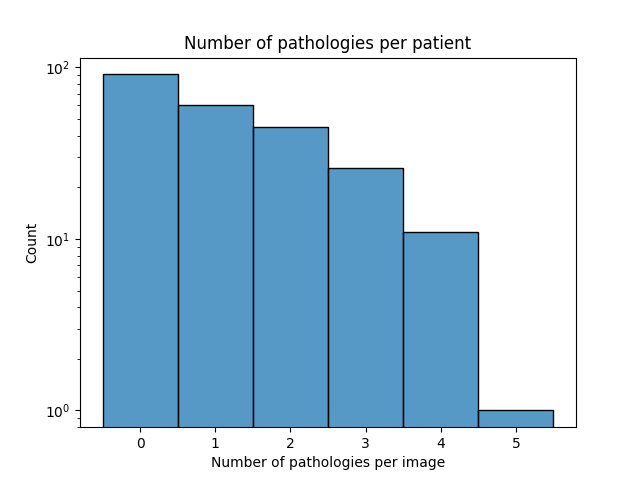
\includegraphics[width=\linewidth]{plots/disease_count_chexpert_valid}
         \caption{CheXpert's validation dataset}
         \vspace{4ex}
         \label{fig:count_chexpert_valid}
     \end{subfigure}
     \label{fig:classes_per_image}
     \caption{Histogram for the different labels present in the CIUSSS and CheXpert dataset}

\end{figure}
    
    \newpage
\begin{figure}[H]
     \centering
     \begin{subfigure}[b]{0.45\linewidth}
         \centering
         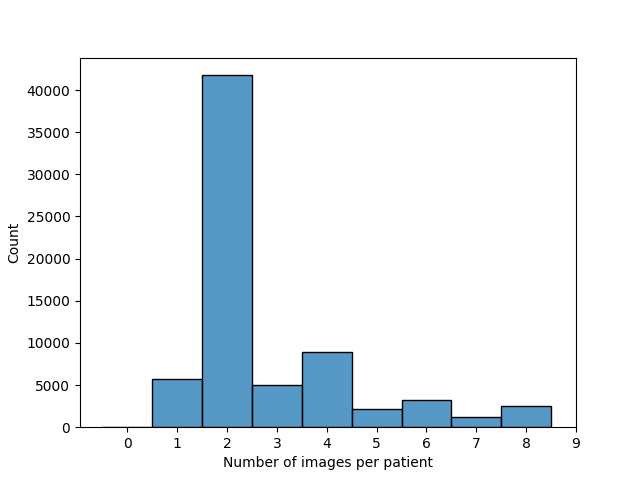
\includegraphics[width=\linewidth]{plots/image_count_ciusss_train}
         \caption{CIUSSS's training dataset}
         \vspace{4ex}
         \label{fig:count_image_ciusss_train}
     \end{subfigure}
     \hfill
     \begin{subfigure}[b]{0.45\linewidth}
         \centering
         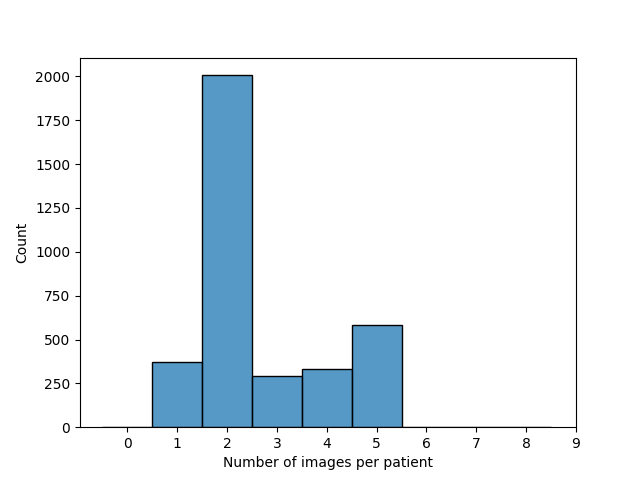
\includegraphics[width=\linewidth]{plots/image_count_ciusss_valid}
         \caption{CIUSSS's validation dataset}
         \vspace{4ex}
         \label{fig:count_image_ciusss_valid}
     \end{subfigure}


     \begin{subfigure}[b]{0.45\linewidth}
         \centering
         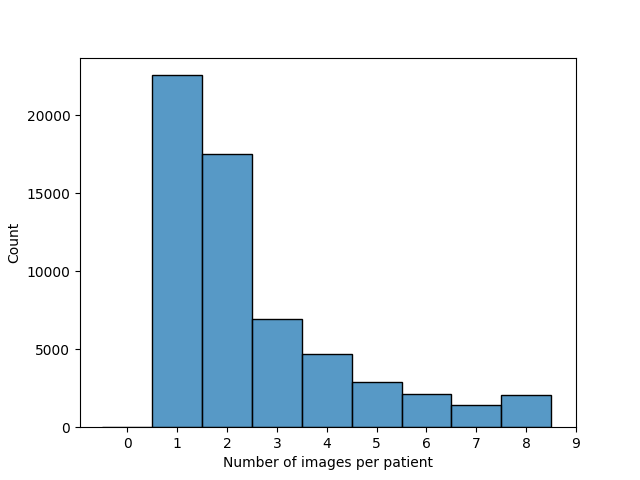
\includegraphics[width=\linewidth]{plots/image_count_chexpert_train}
         \caption{CheXpert's training dataset}
         \vspace{4ex}
         \label{fig:count_image_chexpert_train}
     \end{subfigure}
     \hfill
     \begin{subfigure}[b]{0.45\linewidth}
         \centering
         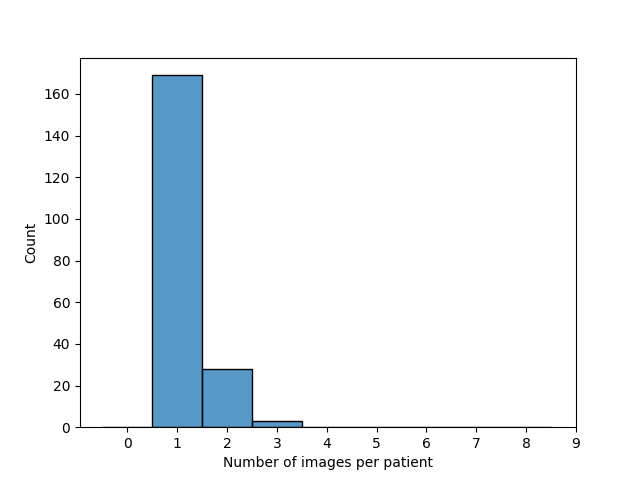
\includegraphics[width=\linewidth]{plots/image_count_chexpert_valid}
         \caption{CheXpert's validation dataset}
         \vspace{4ex}
         \label{fig:count_image_chexpert_valid}
     \end{subfigure}
     \label{fig:images_per_patient}
     \caption{Histogram for the number of images per patient present in the CIUSSS and CheXpert dataset}

\end{figure}

   

    As mentionned earlier, the data is unbalanced! While typically , we would simply undersample the overrepresented
    categories or the opposite, oversample the under-represented classes, it is not an option here. Looking closely at the data~\ref{fig:classes_per_image},
    we can see our problem is not a simple classification, but a multilabel classification tasks where more than one class might be present
    in the input. We also see that we have a lot of images with no pathology at all in the CCSMTL dataset. This is a 
    problem as it means that the model will be biased toward answering no pathology are present. We therefore need 
    to undersample this category!



    To resolve the imbalancy, we can also assign each positive example of a class with a weight, therefore increasing the importance of the positive examples of the under-represented classes. This is
    done by using the class weights parameter of the loss function. This is a good solution, but it is not perfect of course as one class might have a higher preponderance in the loss
    function.
    
    Secondly, our data does not come in the form of a simple image. The input is composed of multiple images present 
    in the patient file for a specific exam, typically between 1 and 4 images~\ref{fig:images_per_patient}. While a RNN could be use to deal
    with a sequence of image, no such model exist for medical imaging. Instead, we will use a CNN to process each image independently, and combine the output with a simple addition before applying the sigmoid activation function.

    To further simplify the model, we also explored two other option

    \subsection{Option 1 : Only use 1 frontal image}
        Our first attempt was to use only one frontal image per patient. This is a simple solution, but it is not optimal as it does not take into account the other images present in the patient file.
        However, we quickly realize that this was not a good idea as the model was underperforming with some specific pathologies. This was most
        likely due to these pathologies having been identified through the other images present in the patient file, and especially the lateral images.
        Further investigation confirmed our hypothesis, as some pathologies like pleural effusion were mostly confirmed by the lateral images.

    \subsection{Option 2 : Use two different set of weights for the feature extraction of frontal vs lateral images}

        To ensure the model learned in an optimal manner from both lateral and frontal images, we tried to use two different set of weights for the feature extraction of frontal vs lateral images. This however
        effectively double the number of parameters to train, and led to a significant increase in the model capacity and overfitting. This option was therefore also rejected.

        % link to document?
    Finally , we opted to use two of the images present in the patient file, and to combine the output of the CNN with a simple addition before applying the sigmoid activation function. This is a simple solution, but it is not optimal as it does not take into account the other images present in the patient file.
    It however will help simplify training as the model will almost always have the same number of input images (2, more rarely 1), and will also help with the generalization of the model as it will be trained on a wider variety of images.

    To undersample the empty images, we will ponder them with a weight of 0.1, and the other images with a weight of 1. This will effectively leave us with a dataset containing the equivalent of only about 20 000 empty images.


    \section{Preparing the data}

    \myworries{Should we talk about the conversion from DICOM to PNG?}

    Before sending our data into a machine learning algorithm , we need to think about the preprocessing that we can
    apply on it to facilitate the learning process. For our use case, with deep learning models, it is typical to
    split this step in two part : augmentations and normalization.


    For data augmentations, we used a combination of random horizontal flipping of the image, as the lungs are symmetrical,color jittering, to add random noise
    in the images, affine transformation (see albumentation's documentation \footnote{https://albumentations.ai/docs/api_reference/augmentations/geometric/transforms/}), and a mix of griddistortion and Elastic transformation to simulate a greater
    variance in the shape of the specified pathologies. All the augmentations were done with Albumentations, as to avoid making mistakes
    by writing our own\cite{albumentations}. The detail of the augmentations :

    \begin{itemize}
        \item \textbf{Affine} : randomly apply affine transformations : translation, rotation, shear and scale with
        probobility $p_0$. The translation is done with a maximum of 15\% of the image's width and height, the
        rotation is done with a maximum of 25 degrees and a translation of up to 15\% is also done.
        \item \textbf{ColorJitter} : randomly change the brightness, contrast and saturation of the image with
        probability $p_1$, and a maximum of 0.2 for each of the three parameters.\footnote{While it may sound strange
        to apply color jittering on a grayscale image, it is still possible to apply it, as it will simply affect the
        contrast, brightness and saturation of the image.}
        \item \textbf{HorizontalFlip} : randomly flip the image horizontally with probability $p_2$
        \item \textbf{GridDistortion} : randomly apply grid distortion with probability $p_3$, and the following
        parameters : num\_steps=5, distort\_limit=0.3, interpolation=1, border\_mode=0, value=None, mask\_value=None
        \item \textbf{ElasticTransform} : randomly apply elastic transformation with probability $p_4$, and
        parameters : alpha=0.2,sigma=25 and alpha\_affine=50
        \label{tab:augmentations}
    \end{itemize}

    Data augmentation such as this serves two purposes. The first one is to allow the model to generalize better, as it is given
    a wider variety of examples (albeit partially synthetic examples) . The second purpose is to avoid overfitting as the model will
    have a harder time simply memorizing the examples instead of actually learning the desired characteristic within the image.

    The second step, normalization, serves to assure that the distribution of the image stay within a specified norm. It is typical
    to bring the images values between 0 and 1, and , if using a pretrained model as it is our case, to normalize the data
    according to the specified mean and standard deviation value of the images used to pretrain the model (in our case ImageNet).

    It is also possible to use histogram equalization. This method will normalize image with respect to local values instead of the global maximum and minimum.
    Improving on this idea we used the Contrast Limited Adaptive Histogram Equalization, an often used method in
    medical imaging~\cite{clahe}
    \footnote{see \url{https://towardsdatascience.com/clahe-and-thresholding-in-python-3bf690303e40}},
    to further improve the normalization and contrast of our images. We hope this will help with the
    cross-generalization of our model on the different datasets.





    \subsection{Dealing with uncertainty labels}



        Since the labels are derived from the radiologist's report, they often include uncertainties express with vocabulary such as \"might\",\"maybe\",\"possible\", etc.
        This is a problem as it is not clear what the label should be. We therefore decided to assign a flag of -1 to all uncertain label (just as it was done with CheXpert). Following this paper~\cite{hierarchical}, which tested different
        ways of dealing with those uncertainty, we replaced uncertain label with a random label sampled uniformly between 0.5 and 0.85, as to imply the label is more likely present than absent if the radiologist
        mentionned it as a possibility.

        This will also act as a form of regularization, as a form of label smoothing \footnote{\url{https://towardsdatascience.com/what-is-label-smoothing-108debd7ef06}}, teaching the model to
        be less overconfident about its prediction. By default, the cross entropy loss will try to minimize the distance between the predicted label and the true label. This is a problem as it will
        put a pressure on the model to simply answer 0 or 1, without leaving much room for uncertainty. If we wish to interpret the
        output of the model as a probability, we need to ensure the model is not overconfident about its prediction. Label smoothing will help with this, as it will teach the model to be less confident about its prediction.

        This will help when communicating with the radiologists, as they will naturally try to interpret the output of the model as a probability. This will also help with the interpretability of the model, as it will
        be easier to explain to the radiologists why the model was wrong, as it should be less confident about its prediction.

        It is important to note that such uncertain label should not and are not in the validation set as to avoid having validation results that include a lot of noise, which would take away a lot of our trust
        in the results.

        Just as with the validation set, the test set should not contain any uncertainty either.
    \section{Model architecture}

    \subsection{Model 1 : DenseNet~\cite{densenet}}


    \begin{figure}[h]

         \centering
         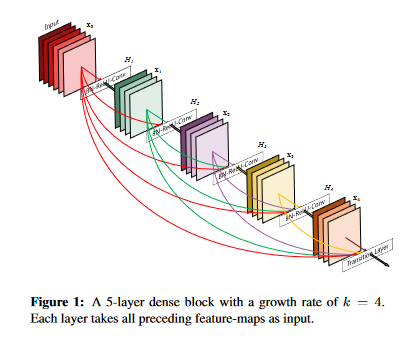
\includegraphics[width=0.5 \textwidth]{plots/densenet_figure}
         \caption{Figure 1 from the densenet paper~\cite{densenet}. It shows how the layers are all interconnected}
         \label{fig:densenet_figure}

    \end{figure}

        The densenet model is a CNN model that is composed of dense blocks. Each dense block is composed of a series of convolutional layers,
        each of which is connected to all the previous layers in the block (see~\ref{fig:densenet_figure}). This allows the model to learn features at different scales, and to
        combine them in a more efficient manner. The model is also composed of a transition layer, which is used to reduce the number of feature maps
        and to control the growth of the model. The model is also composed of a classifier, which is composed of a global average pooling layer and a fully connected layer.



        This model released in 2018 improved on ResNet with its dense blocks, and was the state of the art for a while. The stanford team working on ChexNet found it was the best model available to achieve the highest AUC on CXR images~\cite{chexnet}.


    \subsection{Model 2 : ConvNeXt~\cite{convnext}}


\begin{figure}[H]

     \centering
     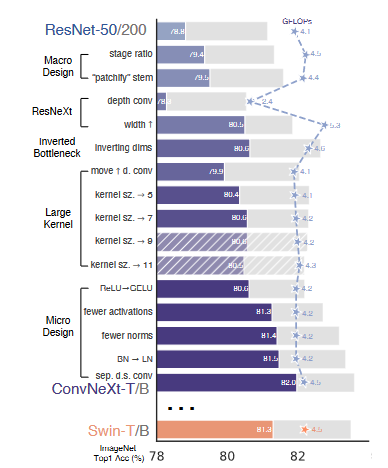
\includegraphics[width=0.5 \textwidth]{plots/convnext_graph}
     \caption{Figure 2 from the ConvNeXt paper~\cite{convnext}. It details the different improvement made to the
     resnet architecture and the gain in performance obtained following each modification.}
     \label{fig:convnext}

\end{figure}

        The ConvNeXt model is another CNN model, this time released in 2020 and improving on the default Resnet architecture once again.
        They gradually implemented many of the features of vision transformers in order to \"modernize\" the typical
    CNN architecture. In doing sp,
        they created an architecture which outperformed many SOTA models on the ImageNet competititon.

        The details of these modifications can be seen in the figure~\ref{fig:convnext}, which is taken from their paper.
        It replaced densenet as the \"default\" convolutionnal model


    \subsection{Model 3 : EfficientNet~\cite{efficientnet} and YOLO~\cite{yolo}}


\begin{figure}[H]

     \centering
     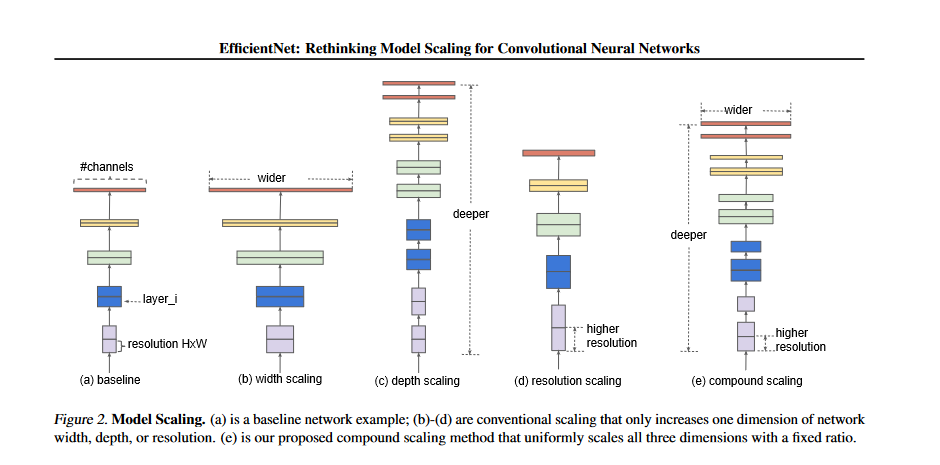
\includegraphics[width=0.8 \textwidth]{plots/efficientnet}
     \caption{Figure 2 from the ConvNeXt paper~\cite{efficientnet}. It shows the different approach that deep learning
     model can take to model scaling, compared to their version.}
     \label{fig:efficientnet}

\end{figure}

    EfficientNet was another model improving on the basic building blocks of CNN, in order to improve the efficiency (see~\ref{fig:efficientnet}). While it is
    not the best one, this approach has led to further development. Such improvement came in the form of the You Only Look Once (YOLO) object detection
    model, which quickly became a SOTA model. Further improvement have allowed this model to keep its position as one of the best pretrained model publicly available.

    \subsection{Model 4 : Deit \& Transformers~\cite{deit}~\cite{image16x16}}


        \begin{figure}[H]

             \centering
             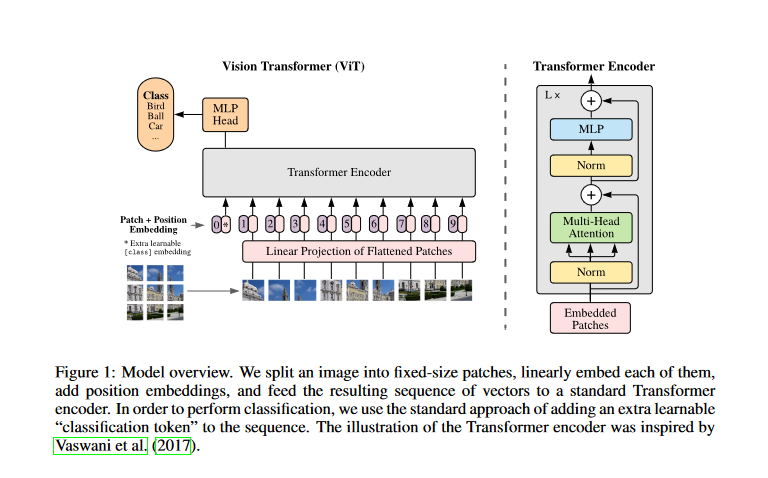
\includegraphics[width=0.8 \textwidth]{plots/transformer}
             \caption{Figure 1 from the An image is worth 16x16 words paper~\cite{image16x16}. It shows the general approach of an image transformer.}
             \label{fig:transformer}

        \end{figure}

        Transformers are a new revolution in deep learning. First developped to deal with natural language processing (NLP),
        they were later introduced in image models, successfully improving on CNN's. While CNN still keep a few key
        elements on their side(they usually perform better to extract local information in an image), transformers split the image in blocks,
        treating them as different element of a sequence (see~\ref{fig:transformer}). Among other things, this allows them to better extract global feature present in an image.

        Later, the facebook research team improved on this general idea by pretraining the model on a similar, but different task, a now
        common approach when using transformers. This allowed them to achieve a greater accuracy in the ImageNet competiton than previous models.


    \section{Training}


    \subsection{Loss function}
        To train a classification model with a multilabel output, we use the Binary Cross Entropy. We therefore treat
        each class as a binary classification problem.

        To account for our dataset imbalance, we will also use weights for the positive example of a class ($P_c$), and weights for the specific classes ($w_c$) such that the loss will be

        \begin{equation}
            L = \frac{1}{N}\sum_{n=0}^N -w_n[p_c y_n log(\sigma(x_n)+(1-y_n) log(1-\sigma(x_n)))]
        \end{equation}

    \subsection{Learning Rate Scheduler}

        We will use a learning rate scheduler to help the model converge faster. We will use a OneCycle learning rate~\cite{onecyclelr}, which will
        decrease the learning rate as the training progresses. This should help the model converge better, as it will first allow it to explore a more vast
        parameter space, before allowing it to converge into a local minimum.

    \subsection{Early stopping}

        Early stopping is a technique used to avoid overfitting. It consists of stopping the training when the validation loss starts to increase. We will
        implement a patience mechanism so that the training will stop only if the validation loss has not improved for a certain number of epochs.
    \subsection{Optimizer}

        Multiple optimizer exists, building on one another . While none is perfect, or definitely better than another, AdamW~\cite{adamw} \footnote{See \url{https://pytorch.org/docs/stable/generated/torch.optim.AdamW.html}} is oftenly use as it tends
        to converge rapidly, thus allowing for far smaller training time.

        AdamW is a slightly modified version of the optimizer Adam (which itself is a modified version of AdaGrad and RMSProp), and fixed an error in the L2 regularization from the original implementation.

        AdamW is also chosen as it has demonstrated its abilities to converge easily with the default hyperparameters. This also allows to diminish the needs for finicky hyperparameters tuning.


    \subsection{Experiment Tracking}
        To track our experience, we used Weight\&Biases\footnote{\url{www.wandb.ai}} .This tool allows us to track the different hyperparameters,
        the loss, the accuracy, and the model architecture. It also allows us to compare different runs, and to easily reproduce them.
        W\&B also allows us to easily upload our model to their servers, and to download it from anywhere. This
        allows us to easily share our model with other people, and to easily reproduce our results. Finally, it allows us
        to easily run hyperparameters sweeps, which will allow us to find the best hyperparameters for our model once we
        finish our development.

    \subsection{Metrics}
        In any unbalanced dataset, the accuracy won't be enough to determine the performance of a classifier.
        We therefore decided to look into the Area Under the Roc Curve (AUC-ROC) \footnote{\url{https://towardsdatascience.com/understanding-auc-roc-curve-68b2303cc9c5}}
        and the F1-score\footnote{\url{https://towardsdatascience.com/the-f1-score-bec2bbc38aa6}}.


        The F1-score is a metric which combines the precision and the recall, simply written :

        \begin{equation}
            F1 = 2 \times \frac{precision \times recall}{precision + recall}
        \end{equation}

        While the F1-score does allow to evaluate the performance of our classifier, it requires to first assign a
        binary class to our model's output. This in turn require to preset a threshold, which, without the results first, will usually be arbitrarily
        chosen to be 0.5. While this is not ideal, as this arbitrary threshold might hinder our model's performance,
        it is still a good metric to use to evaluate how our model would be received by radiologists.

        On the other hand , the AUC-ROC is a metric which does not require to preset a threshold. It is simply the area under the curve of the ROC curve.
        However, to have a perfect AUC-ROC, our model would have to be overly confident in its predictions, always
        predicting probabilities very close to 0 or 1. While the prediction might be accurate, it makes it harder to
        explain to a radiologist why the model predicted a certain class over another. This is why we will use both
        metrics to evaluate our model's performance.


    \subsection{Classification Head}

        While we use a pretrained model for our feature extraction, leaving us little to change on that side, the classification head is usually a simple fully connected
        layer, allowing us some leniency if we were to want to change it. However, such modification are usually not required for a simple classification model . However , as we switch
        from  classification to object detection, we might want to change this later.

        For now, we might mostly just want to work with the dropout parameter. DropOut is a useful technique to avoid overfitting and increase model
        generalization \footnote{\url{https://towardsdatascience.com/dropout-in-neural-networks-47a162d621d9}}

    \subsection{Tips and Tricks}

    \begin{enumerate}
        \item label-smoothing : A common use technique of adding or removing a small value (e.g 0.1) from the label in
        order to smooth out the gradient (e.g $0\xrightarrow{}0.1$ , $1\xrightarrow{}0.9$ )

        \item batch size : Always use a multiple of 2

        \item Clip-Norm : The weight of the model might sometimes grow larger and larger leading to overflow and
        infinite/Nan values! To avoid this, the gradient's norm might be clipped at a maximum value (e.g 1)

        \item Timm : The code use the timm library~\cite{timm} in order to load a model, allowing
        for an easy use of a multitude of pretrained model.


        \item Input Channels : While models are pretrained to use 3 channels (RGB), we can use a single channel (e.g grayscale). This uses
        only one of the convolution kernel at the first layer of the model, and thus reduce the number of parameters to train. However, it might require more training
        as it will affect the input of all the other layers of the model.

    \end{enumerate}

    \section{Preliminary Results}
        All these results for CheXpert can be found at : \url{https://wandb.ai/ccsmtl2/Chexpert?workspace=user-ccsmtl}
        \subsection{Reproducing CheXpert baseline}
            While we do not have access to the hidden test set from CheXpert, we still have access to their validation dataset. However,
            as can be seen in~\ref{fig:histogram_chexpert_valid}, three classes are not available in the validation dataset. We will therefore have to
            limit our comparison to the classes present in the validation dataset , and to keep in mind our results will
            most likely be higher than they would be on the test set. However, to keep things simple, we will not proceed to model ensembling as this
            will simply put a high computational cost for a simple verification step.

            We will also use positive weight to account for the imbalance of the dataset. The positive weights were calculated using the following formula : $pos\_weight = \frac{N_{neg}}{N_{pos}}$ where $N_{neg}$ is the number of negative samples, and $N_{pos}$ is the number of positive samples for a given class. Their value range
        in between 1 and 95. The values are reported in the table~\ref{table:pos_weight_chexpert}. I suspect that high values might scramble the loss for the batches containing the rare positive samples of that class. We might later want to cap
        the maximum possible value of the positive weight to avoid this.

        While we use a weighted sampler for our dataset,for CheXpert, all the training examples were sampled with equal weights.

            \begin{table}[h!]
                \centering
                \begin{tabular}{@{}lllll@{}}
                \toprule
                Classes          & & & & Weights \\ \midrule
                Opacity          & & & & 1.97    \\
                Air              & & & & 16.76   \\
                Liquid           & & & & 1.16    \\
                Cardiomegaly     & & & & 12.15   \\
                Pleural Other    & & & & 94.76   \\
                Pleural Effusion & & & & 3.07    \\
                Pneumothorax     & & & & 21.06   \\
                Lung Opacity     & & & & 1.68    \\
                Atelectasis      & & & & 9.66    \\
                Lung Lesion      & & & & 27.71   \\
                Pneumonia        & & & & 50.26   \\
                Consolidation    & & & & 33.28   \\
                Edema            & & & & 6.11    \\
                Fracture         & & & & 22.77   \\
                No Finding       & & & & 6.58    \\ \bottomrule
                \end{tabular}
                \caption{Positive weights used for the loss , from the CheXpert dataset}
                \label{table:pos_weight_chexpert}
            \end{table}


            \subsubsection{First Attempt}
            % with pos_weight
                Using everything we describe so far, we obtain results as shown in~\ref{fig:chexpert1_performance}.
                While the model did learned a bit from the data, we are underperforming the baseline by a large margin.
                We will therefore have to try to improve our model.



                \begin{figure}[H]
                     \centering
                     \begin{subfigure}[b]{0.45\textwidth}
                         \centering
                         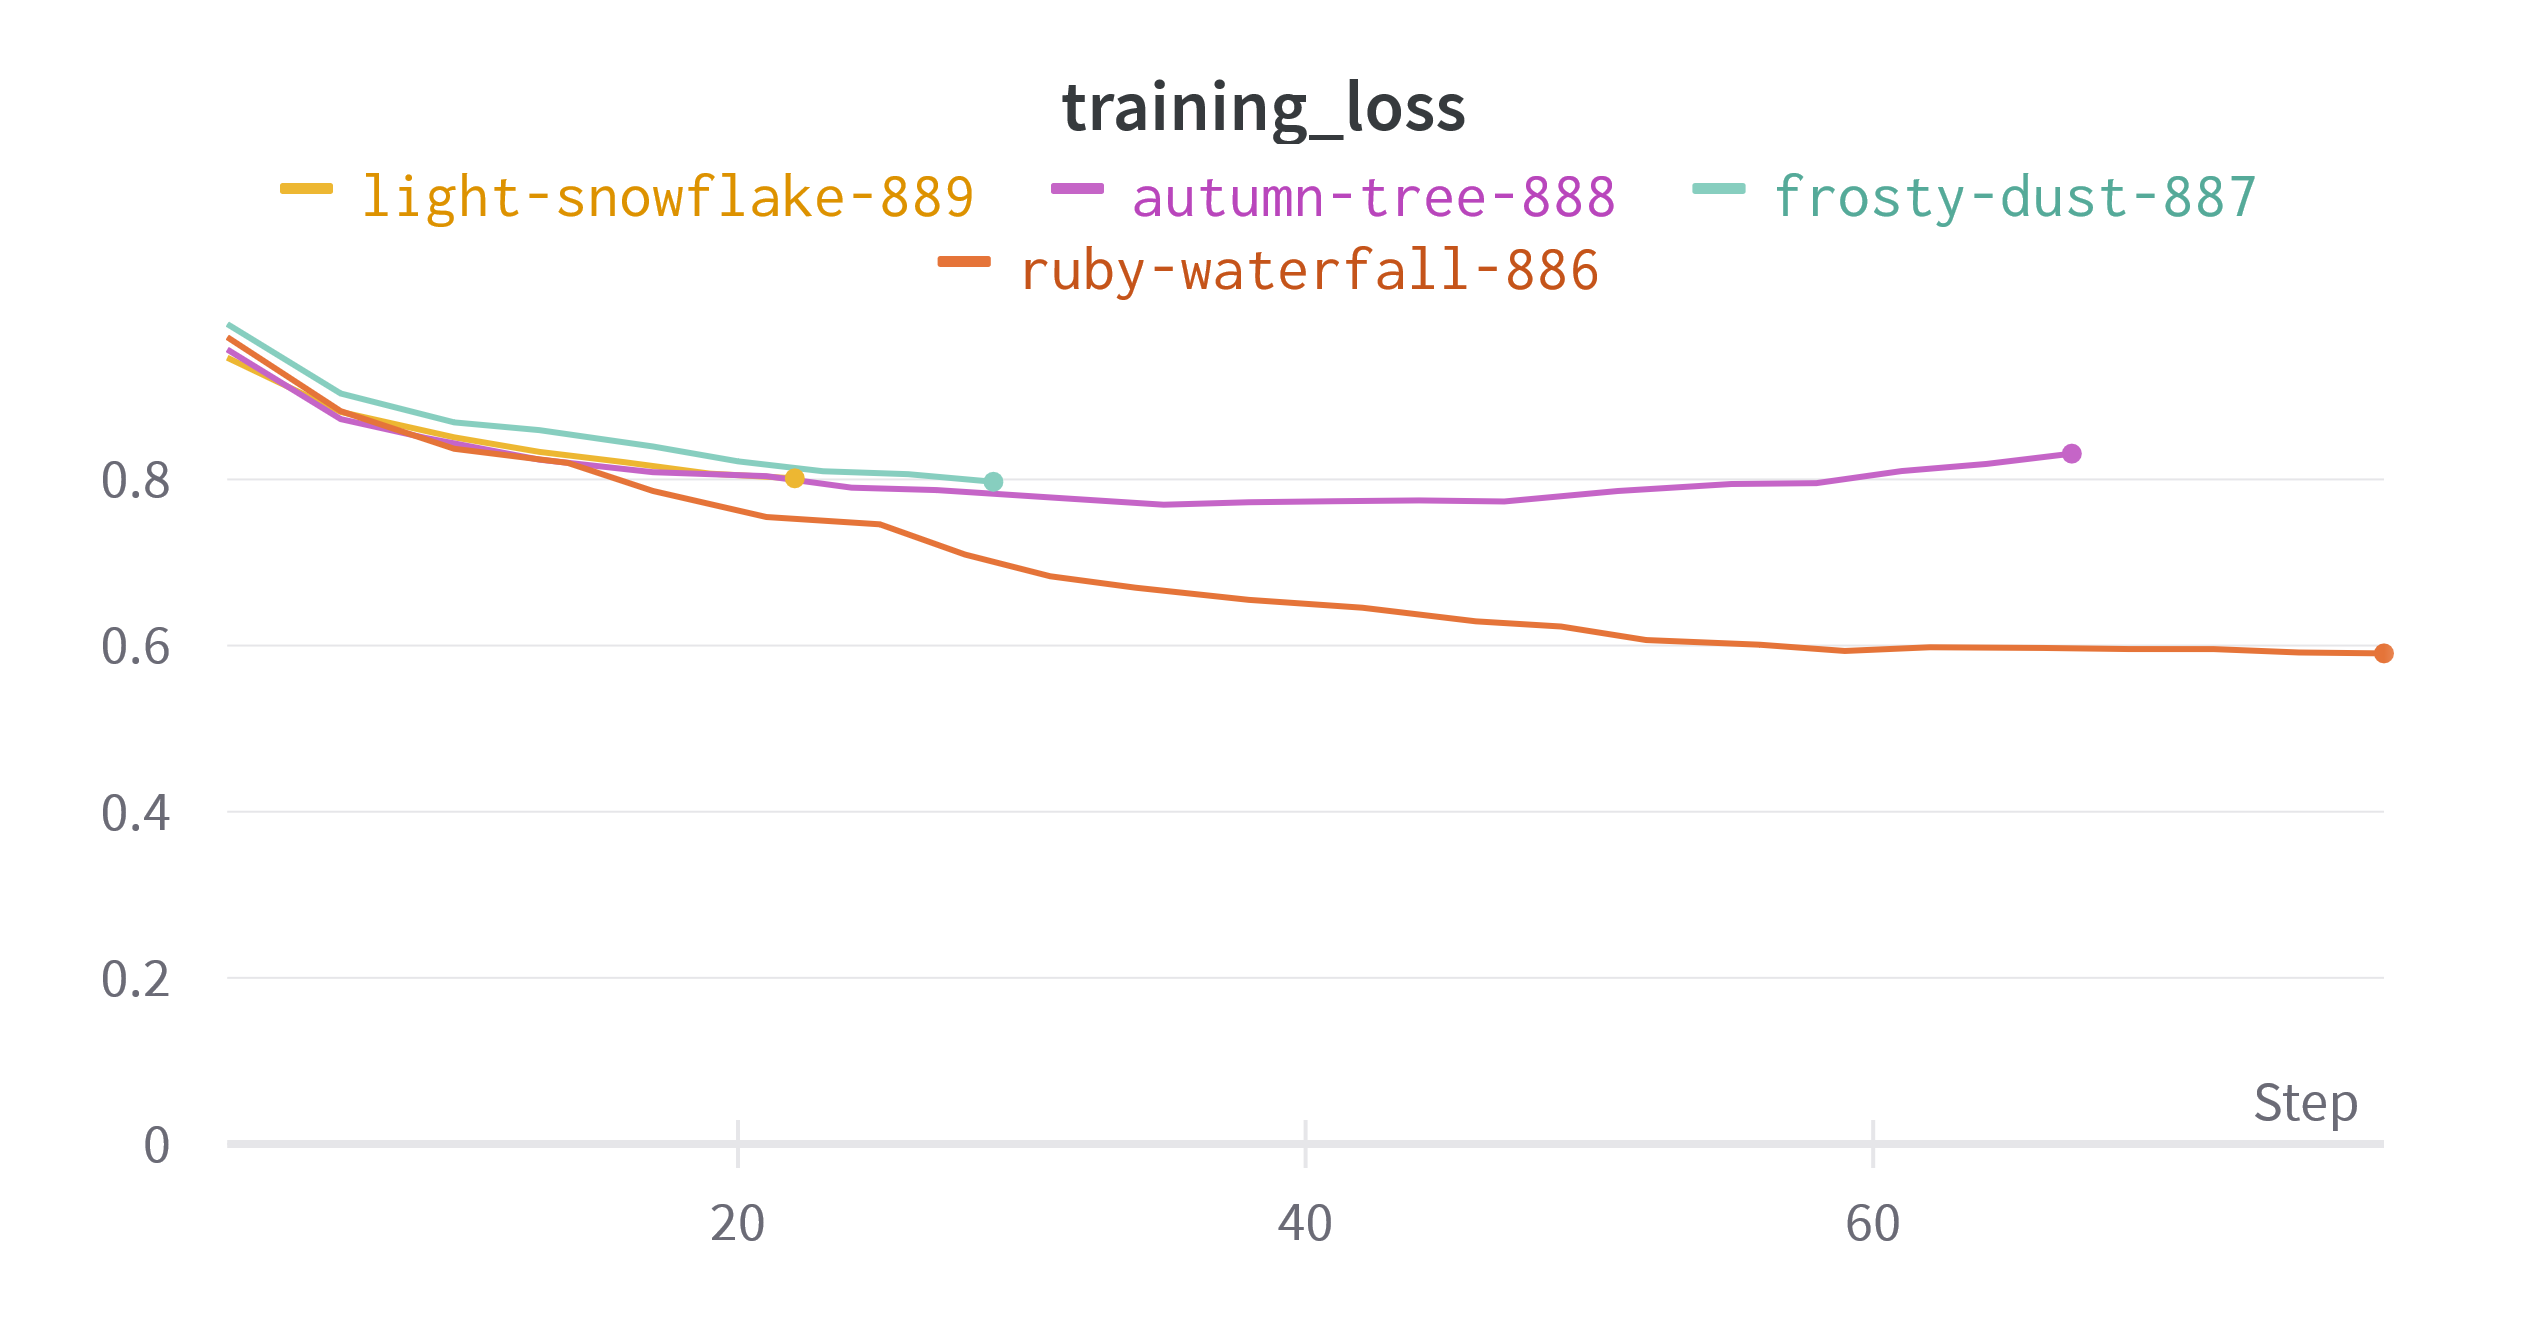
\includegraphics[width=\textwidth]{plots/chexpert_training_loss1}
                         \caption{Training loss}
                         \vspace{4ex}
                         \label{fig:chexpert_training_loss1}
                     \end{subfigure}
                     \hfill
                     \begin{subfigure}[b]{0.45\textwidth}
                         \centering
                         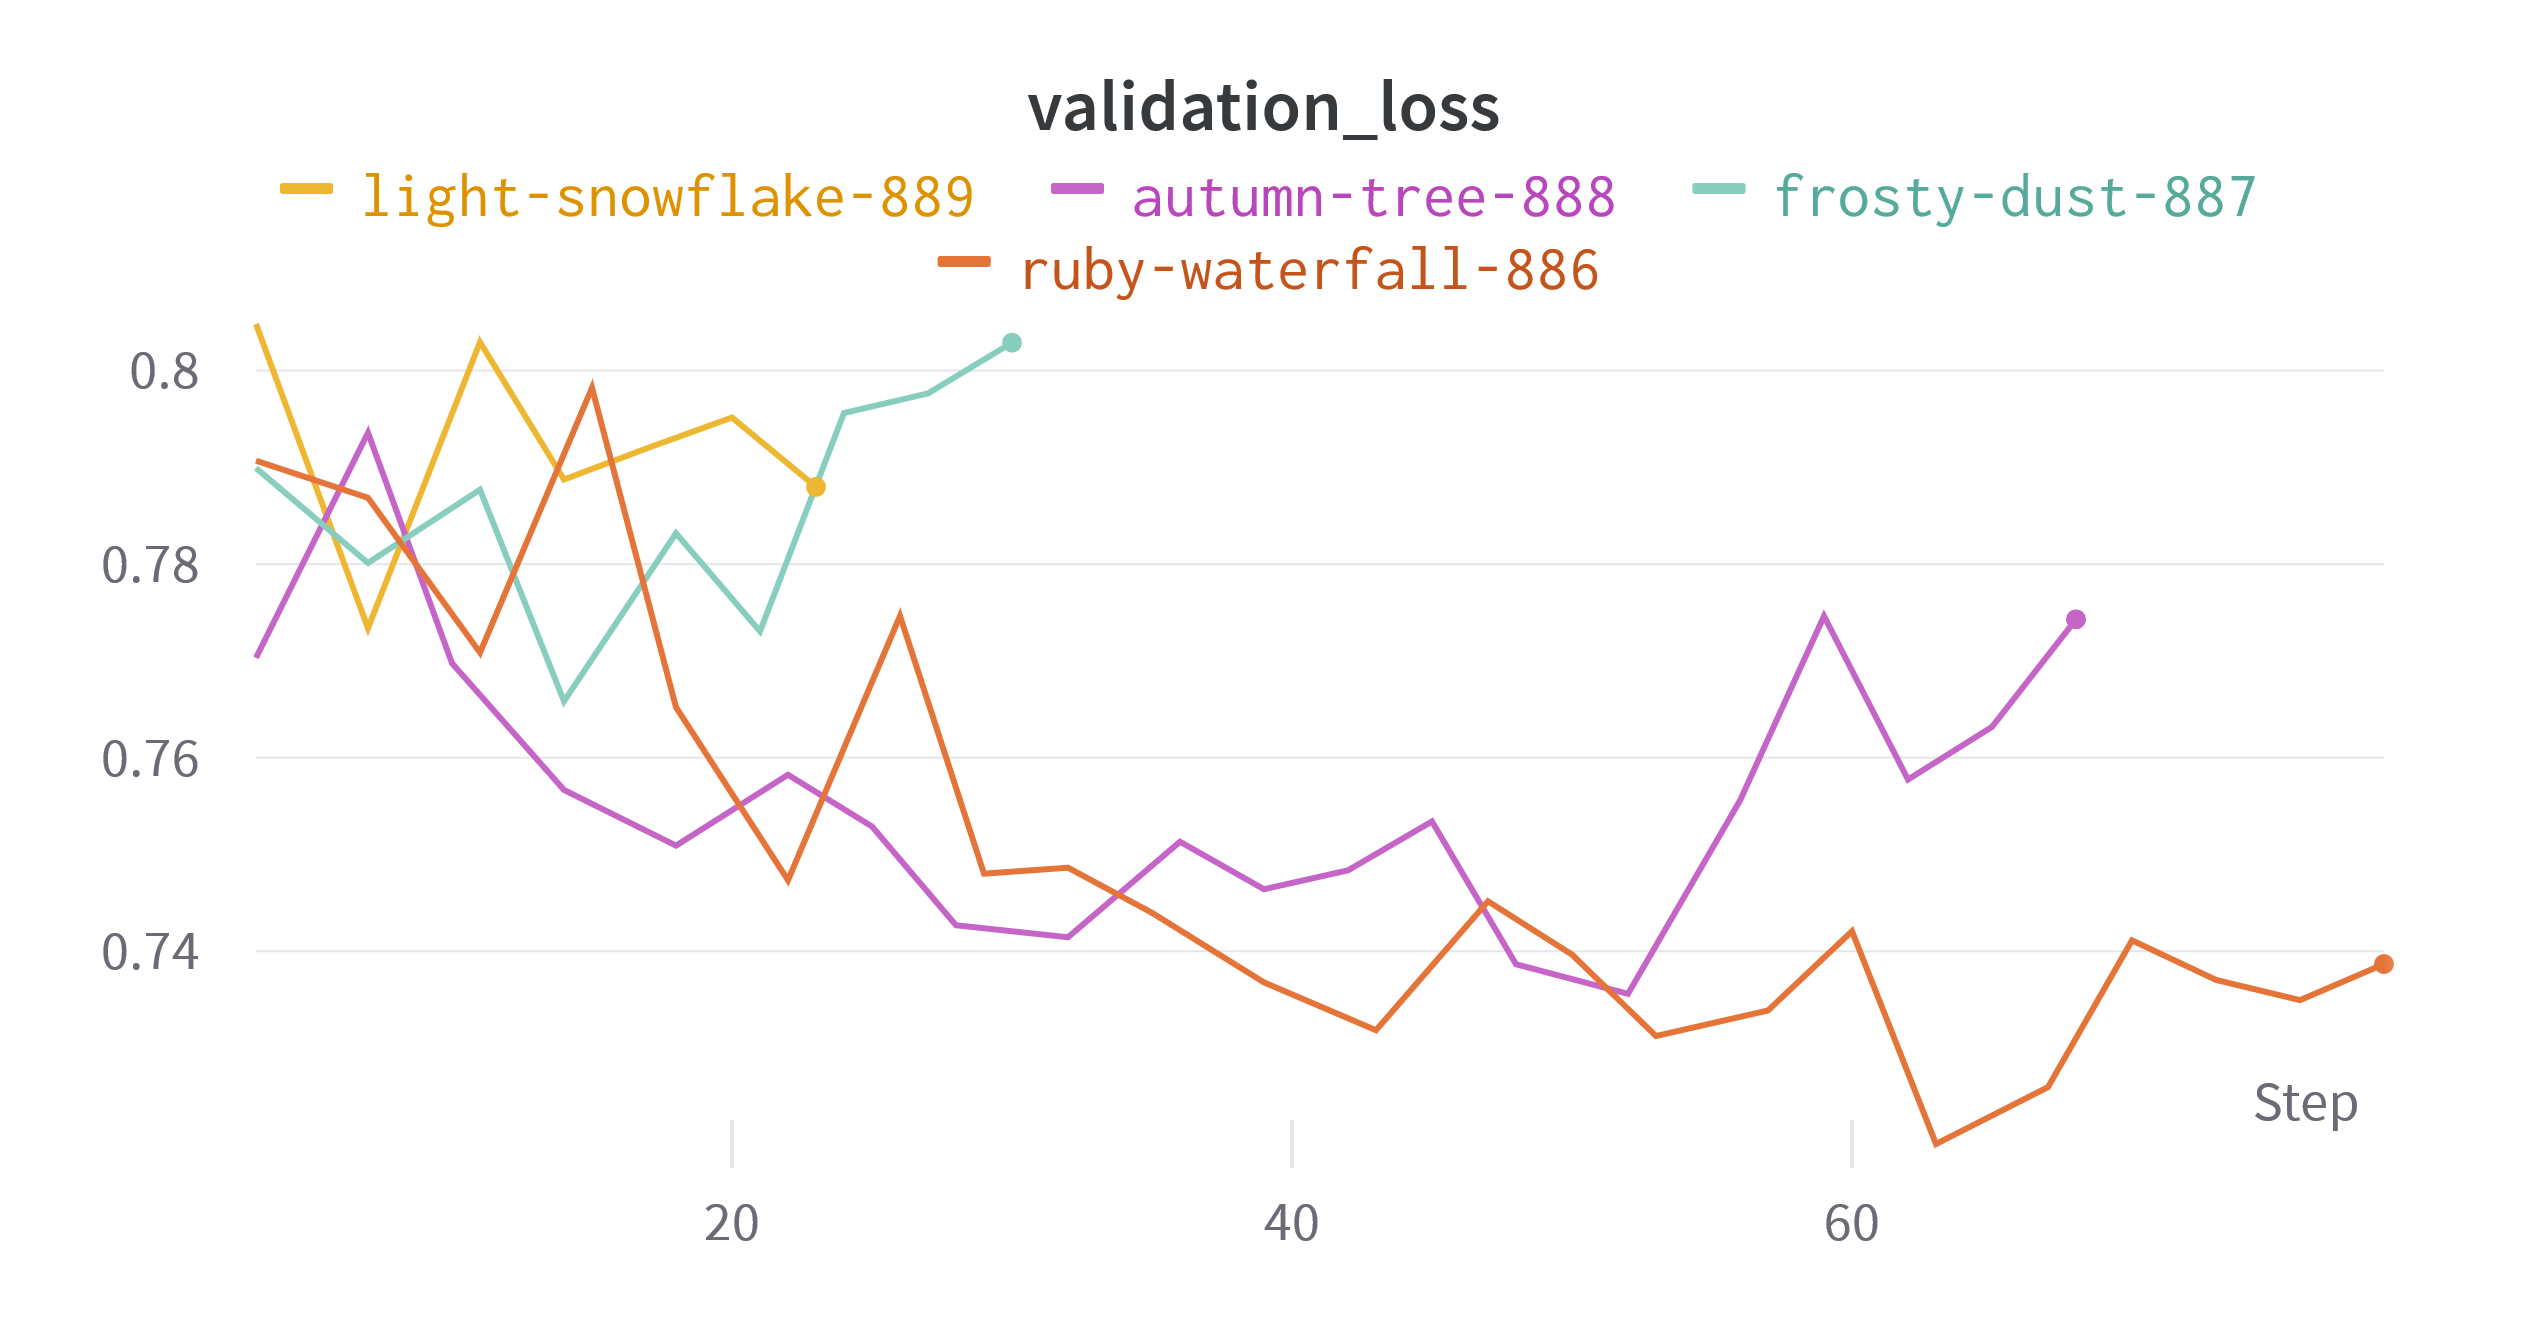
\includegraphics[width=\textwidth]{plots/chexpert_validation_loss1}
                         \caption{Validation loss}
                         \vspace{4ex}
                         \label{fig:chexpert_validation_loss1}
                     \end{subfigure}
                     \label{fig:chexpert_training_curve1}
                     \caption{Training curves for our first attempt at reproducing the CheXpert baseline}
                \end{figure}


                Our second attempt will be at removing the positive weights. Currently, we are only using the weight in the training
                loss. However, this multiplication factor could hide a potential overfit on the training set. Currently, however, it seems the opposite.
                The training loss plateau at around 0.6, while the validation loss varies between 0.8 and 0.6. This would usually indicate that the model
                is underfitting and need to have a bigger capacity.

                Now looking at the f1-score and AUC~\ref{fig:chexpert1_performance}, we can compare the performance of our model to the baseline. We can see that we are underperforming

                \begin{table}[]
                        \centering
                        \begin{tabular}{@{}llllll@{}}
                        \toprule
                        \multicolumn{1}{c}{Classes} &
                           &
                          \multicolumn{1}{c}{\begin{tabular}[c]{@{}c@{}}AUC\\ CheXpert\end{tabular}} &
                          \multicolumn{1}{c}{\begin{tabular}[c]{@{}c@{}}F1-Score\\ (Radiologist's \\ estimation)\end{tabular}} &
                          \multicolumn{1}{c}{\begin{tabular}[c]{@{}c@{}}AUC\\ (Ours)\end{tabular}} &
                          \multicolumn{1}{c}{\begin{tabular}[c]{@{}c@{}}F1-Score\\ (Ours)\end{tabular}} \\ \midrule
                        Cardiomegaly     &  & 0.832 & 0.678  & 0.74 & 0.62 \\
                        Pleural Effusion &  & 0.934 & 0.737  & 0.90 & 0.74 \\
                        Pneumothorax     &  & N/A   & N/A  & 0.87 & 0.23 \\
                        Lung Opacity     &  & N/A   & N/A  & 0.88 & 0.85 \\
                        Atelectasis      &  & 0.858 & 0.692 & 0.71 & 0.63 \\
                        Lung Lesion      &  & N/A   & N/A  & 0.26 & 0    \\
                        Pneumonia        &  & N/A   & N/A  & 0.70 & 0.11 \\
                        Consolidation    &  & 0.899 & 0.385  & 0.85 & 0.41 \\
                        Edema            &  & 0.941 & 0.583  & 0.86 & 0.53 \\
                        No Finding       &  & N/A   & N/A  & 0.84 & 0.93 \\ \bottomrule
                        \end{tabular}
                        \label{fig:chexpert1_performance}
                        \caption{Performance of our first attempt at reproducing the CheXpert baseline. The estimation of the radiologist is the one provided by~\cite{chexzero}}
                \end{table}
                While the  performance for the lung lesion and the pneumonia are not good, we can remember from figure~\ref{fig:histogram_chexpert_valid} that these classes are barely present in the validation dataset (lung lesion only has one image). Ingoring those, we
                find that, while comparing with the AUC, the model has underperformed, we did achieved interesting f1-score. We find that our model seems to perform similarly to a radiologist's on the classes we do have comparisons. This is a good sign, as it means that our model is learning something from the data.

                While our results are slightly lower than the values reported by the CheXpert team, we however achieve close enough value to be confident in our implementation.
                However, only 5 classes were reported in the paper, and we have 10 classes. We will therefore have to compare our results with other sources.

                If you paid attention up to this point, you will also have notice that CheXpert had 14 classes, and not exactly the same as we have!
                This is due to a talk with our radiologist, where they identified some classes as being too similar to be useful, and we thus removed them.


                Rerunning the training without the positive weights, we can now more clearly see that the model is clearly overfitting.
                We should therefore try to switch to model with smaller capacity, and to increase the data augmentation.


            \subsubsection{Second Attempt}
            % without pos_weight
            
                Without the positive weight, as suspected, we can clearly see the overfit of the model~\ref{fig:training_curves2} .
                Our AUC does increase but at the price of a diminished F1-score. This is most likely due to the fact
                that our model as a easier time learning the distribution of positive and negative samples. While it
                helps avoid false positive, it also makes it harder to identify
                the true positive.

                Another interesting thing to remember is that the distribution of positive and negative samples between the training and validation
                dataset is not the same! So while the model can achieve a low loss by simply providing negative answer at first,
                it does not mean that it will be able to generalize to the validation dataset. This is one of the reason why we probably should continue to use
                positive weights.
                %include graphic

                \begin{figure}[H]
                     \centering
                     \begin{subfigure}[b]{0.45\textwidth}
                         \centering
                         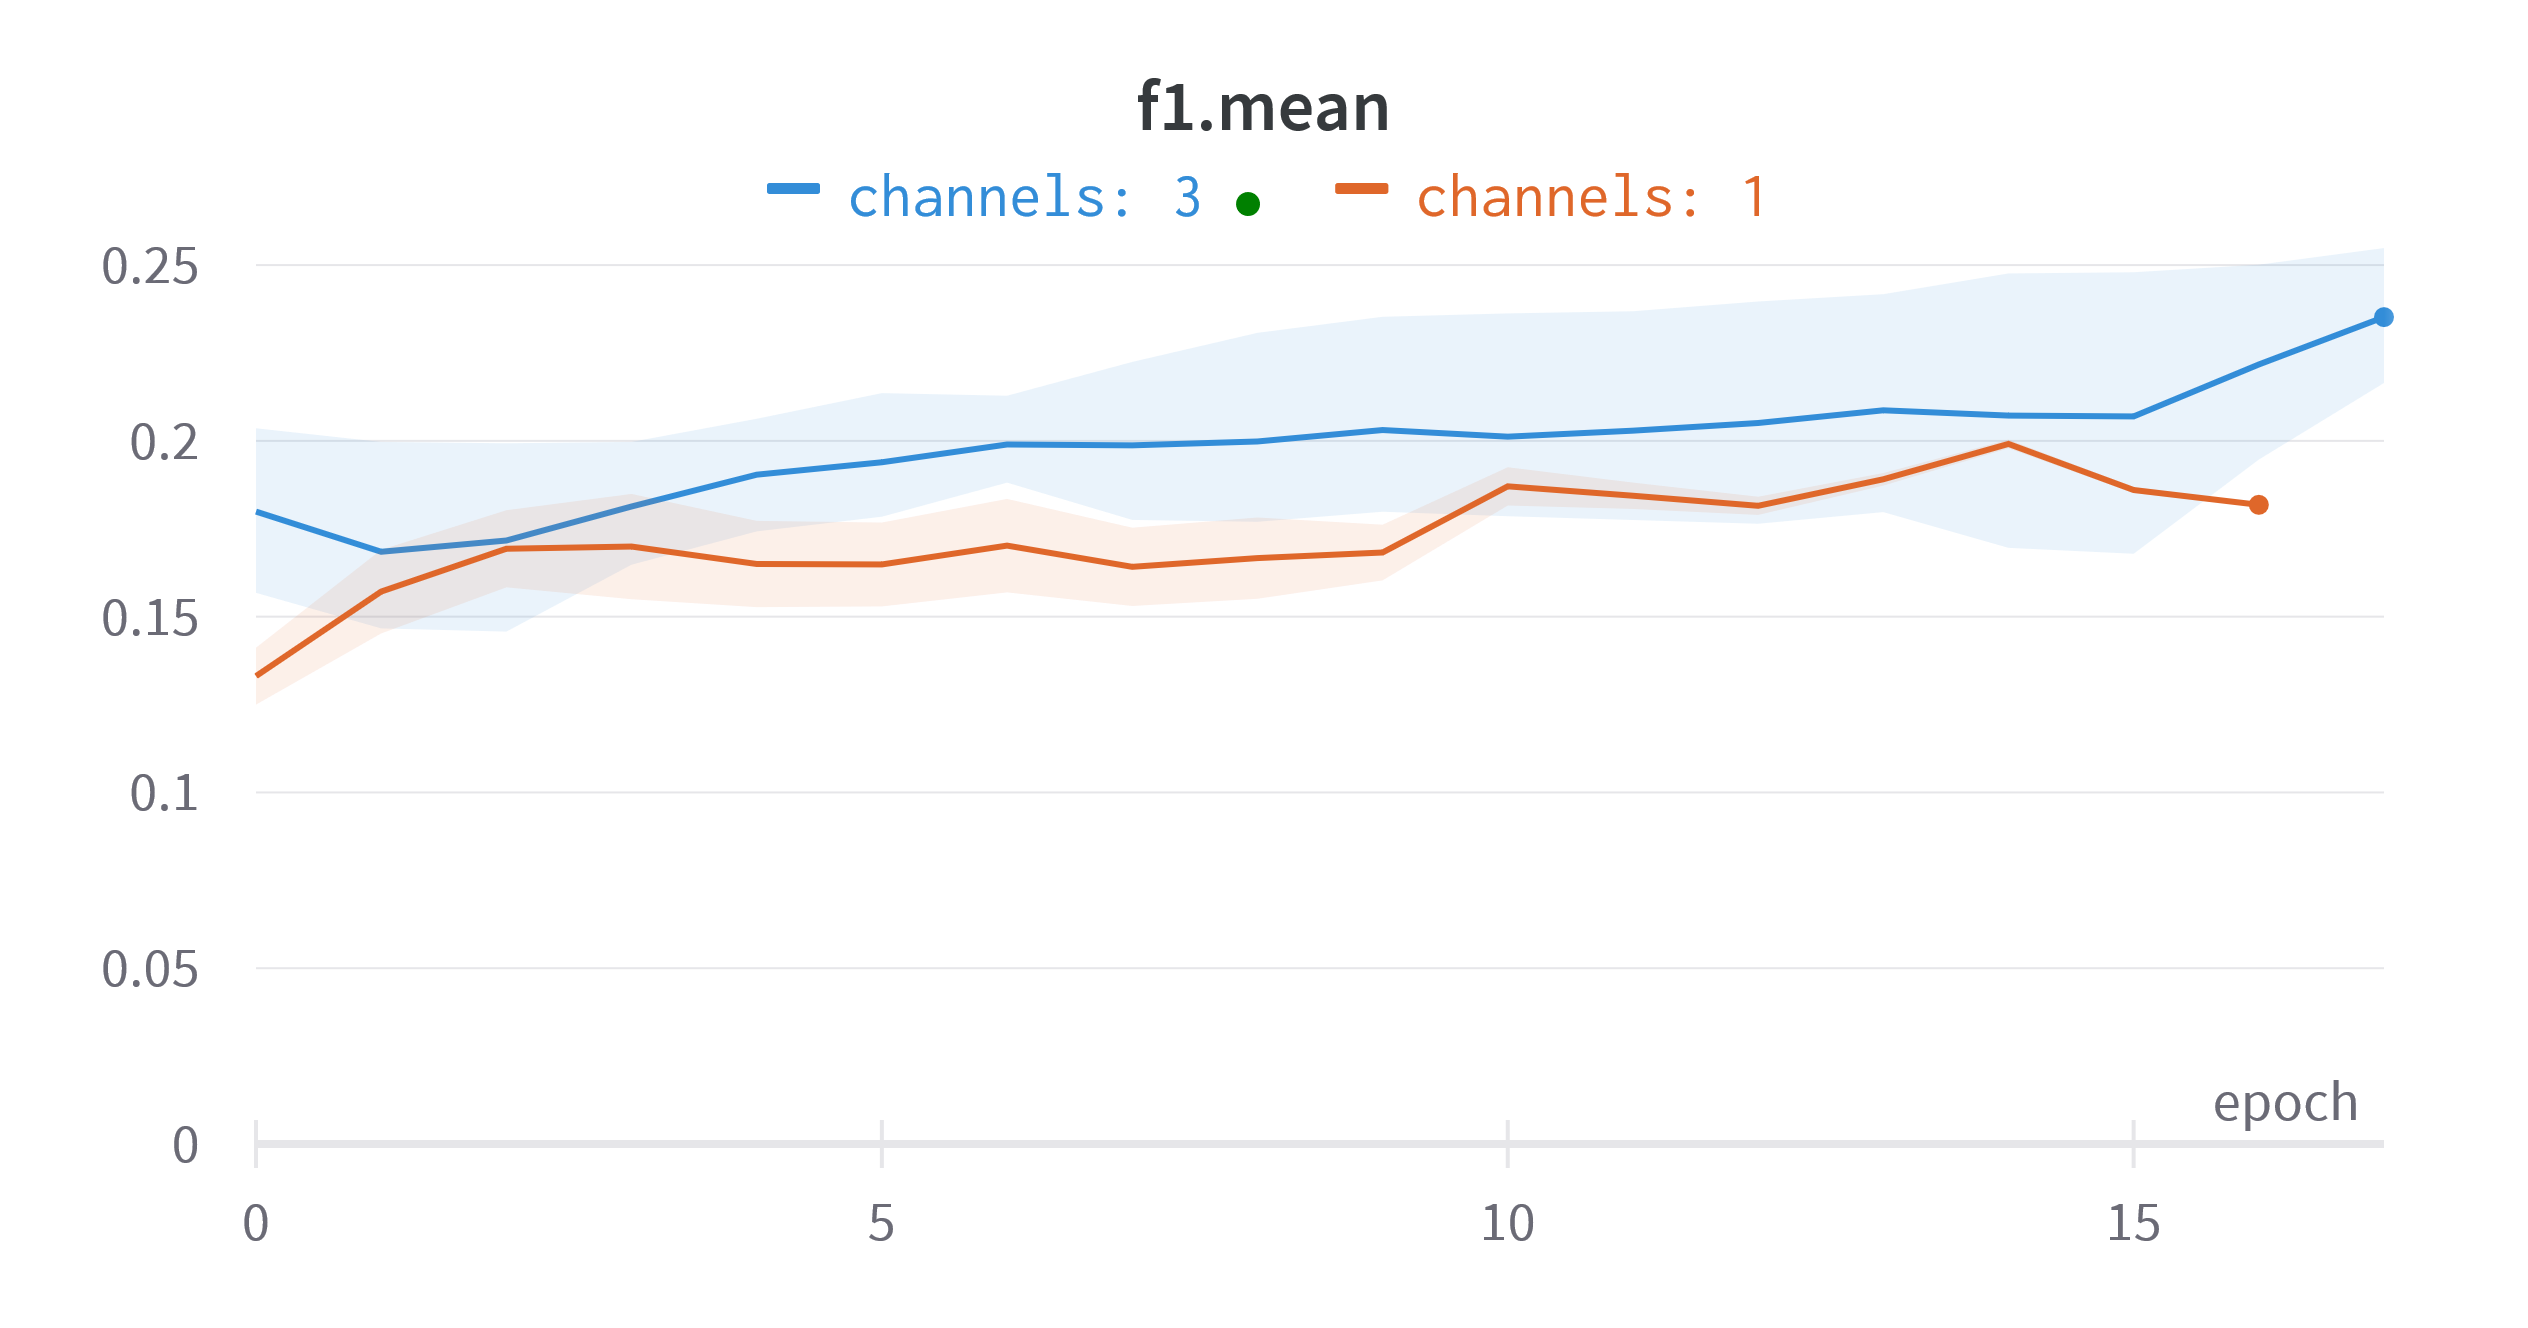
\includegraphics[width=\textwidth]{plots/channel_comparison_f1}
                         \caption{Average f1-score over all classes}
                         \vspace{4ex}
                         \label{fig:channel_comparison_f1}
                     \end{subfigure}
                     \hfill
                     \begin{subfigure}[b]{0.45\textwidth}
                         \centering
                         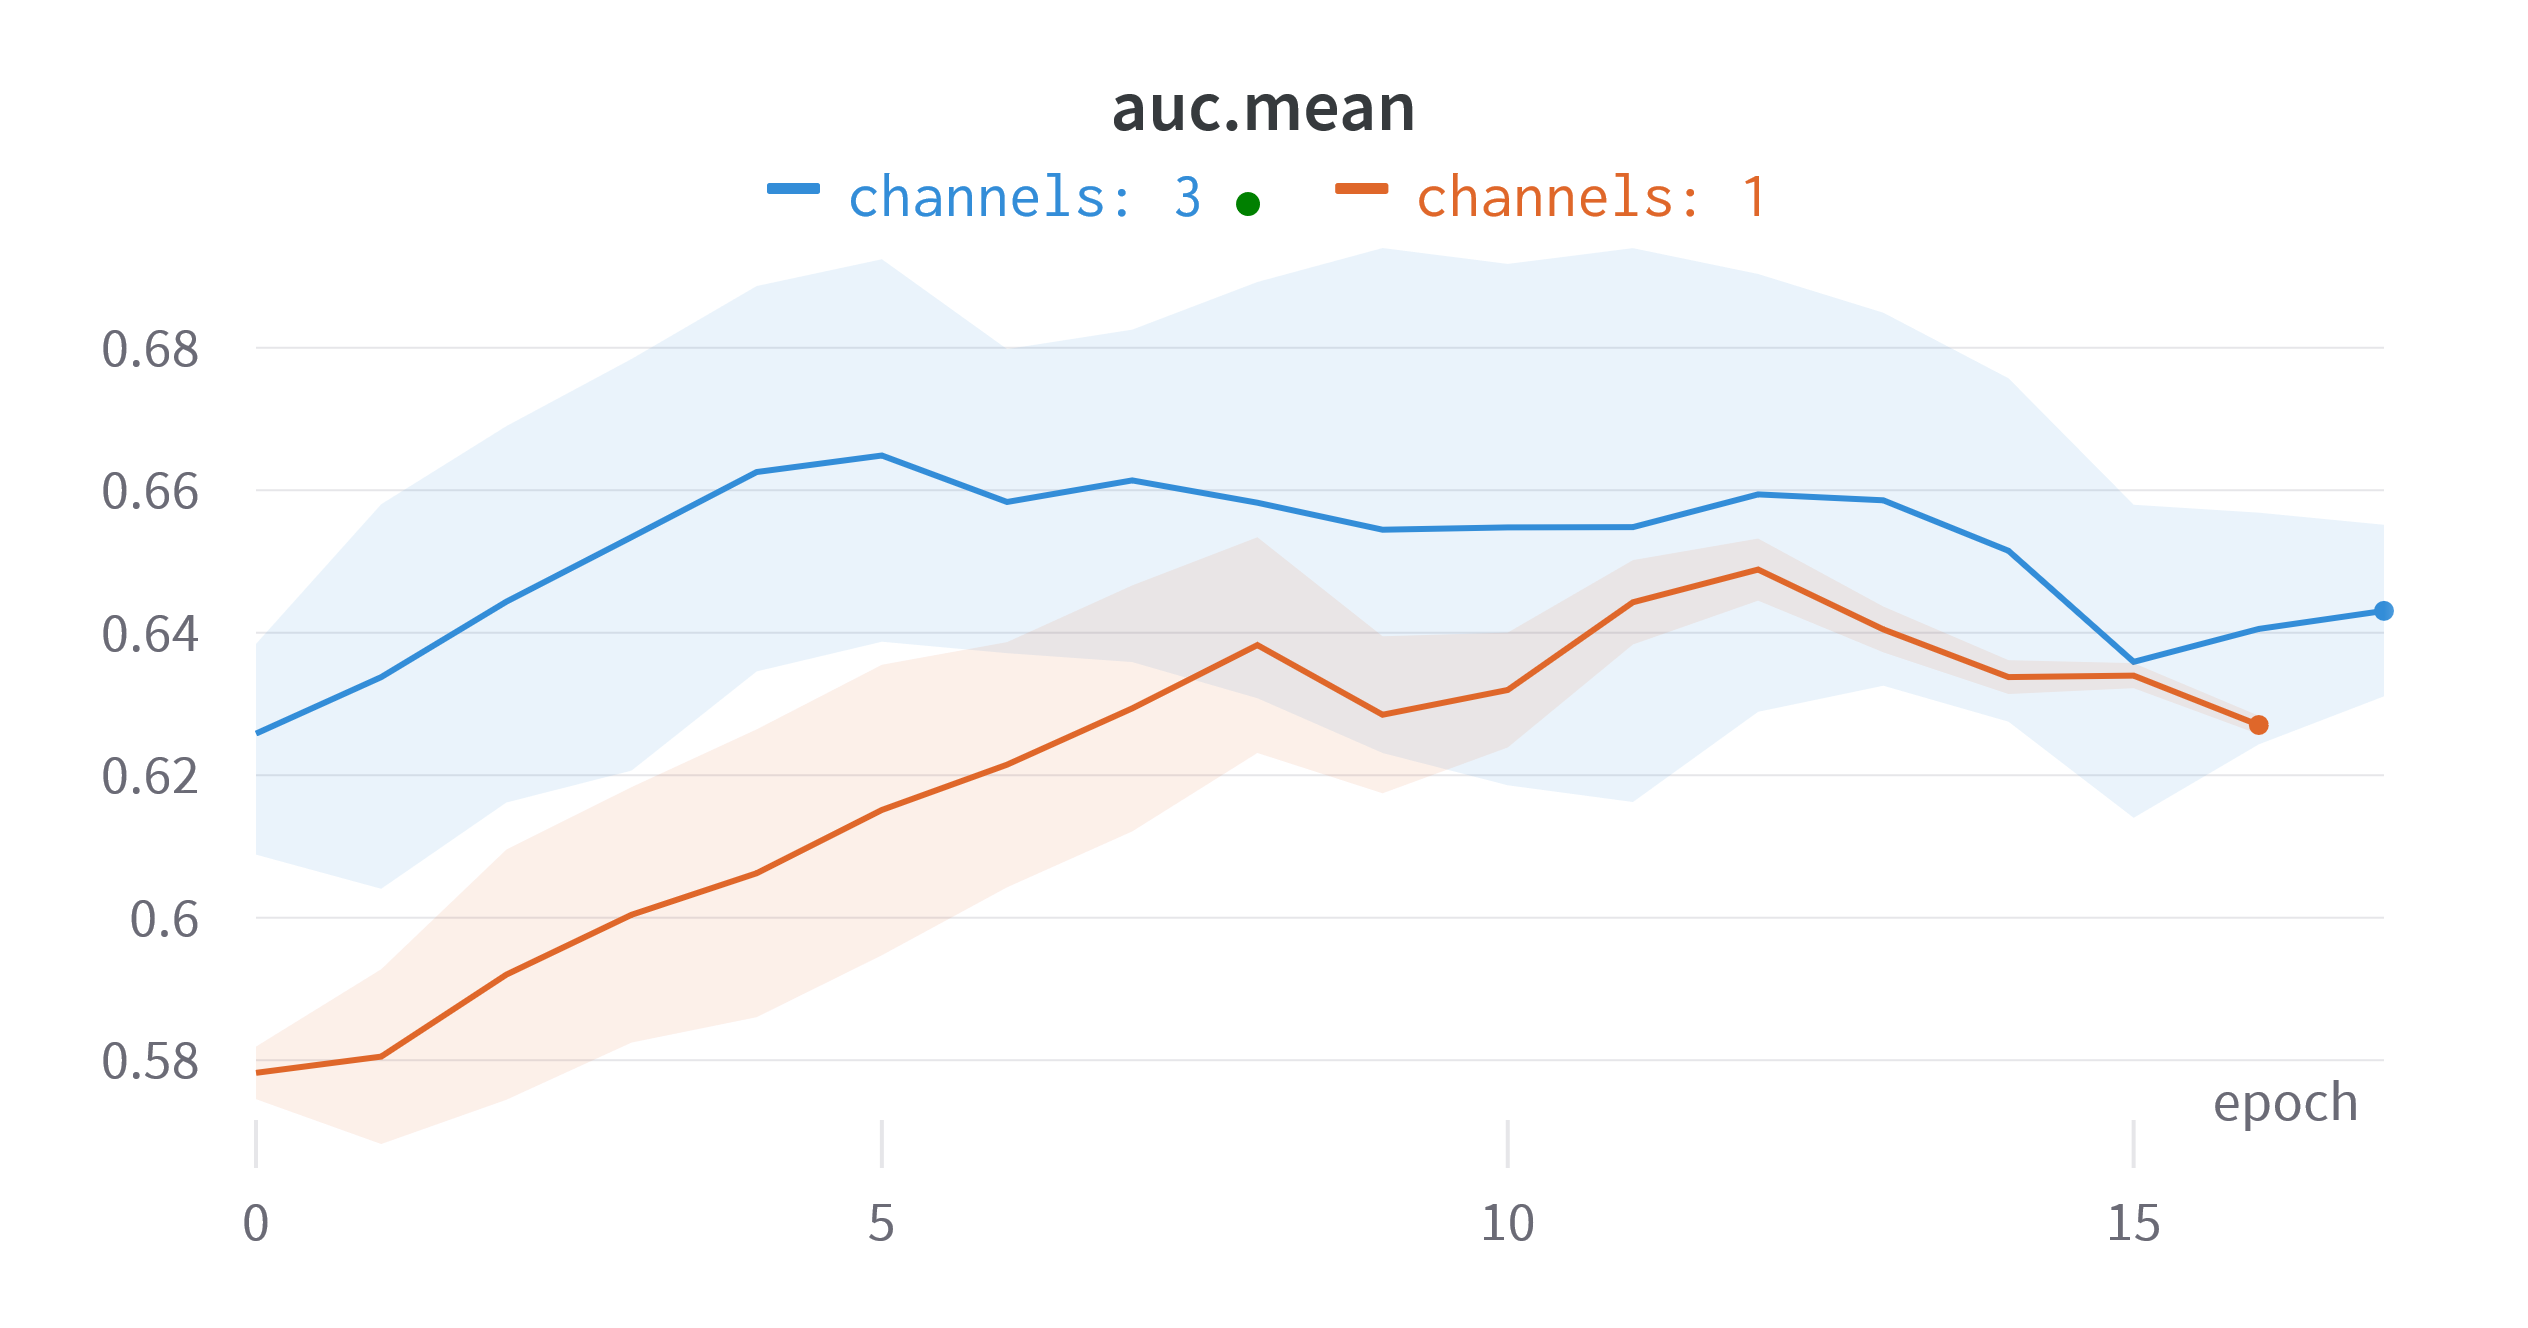
\includegraphics[width=\textwidth]{plots/channel_comparison_auc}
                         \caption{Validation loss}
                         \vspace{4ex}
                         \label{fig:channel_comparison_auc}
                     \end{subfigure}
                     \label{fig:channel_comparison}
                     \caption{Comparisons of the experiments results grouped by number of channels
                         of the input images for the average AUC and f1-score. The curve are smoothed out to help the analysis, and the error bars are the min-max
                         of the values.}
                \end{figure}

                \begin{figure}[H]
                     \centering
                     \begin{subfigure}[b]{0.45\textwidth}
                         \centering
                         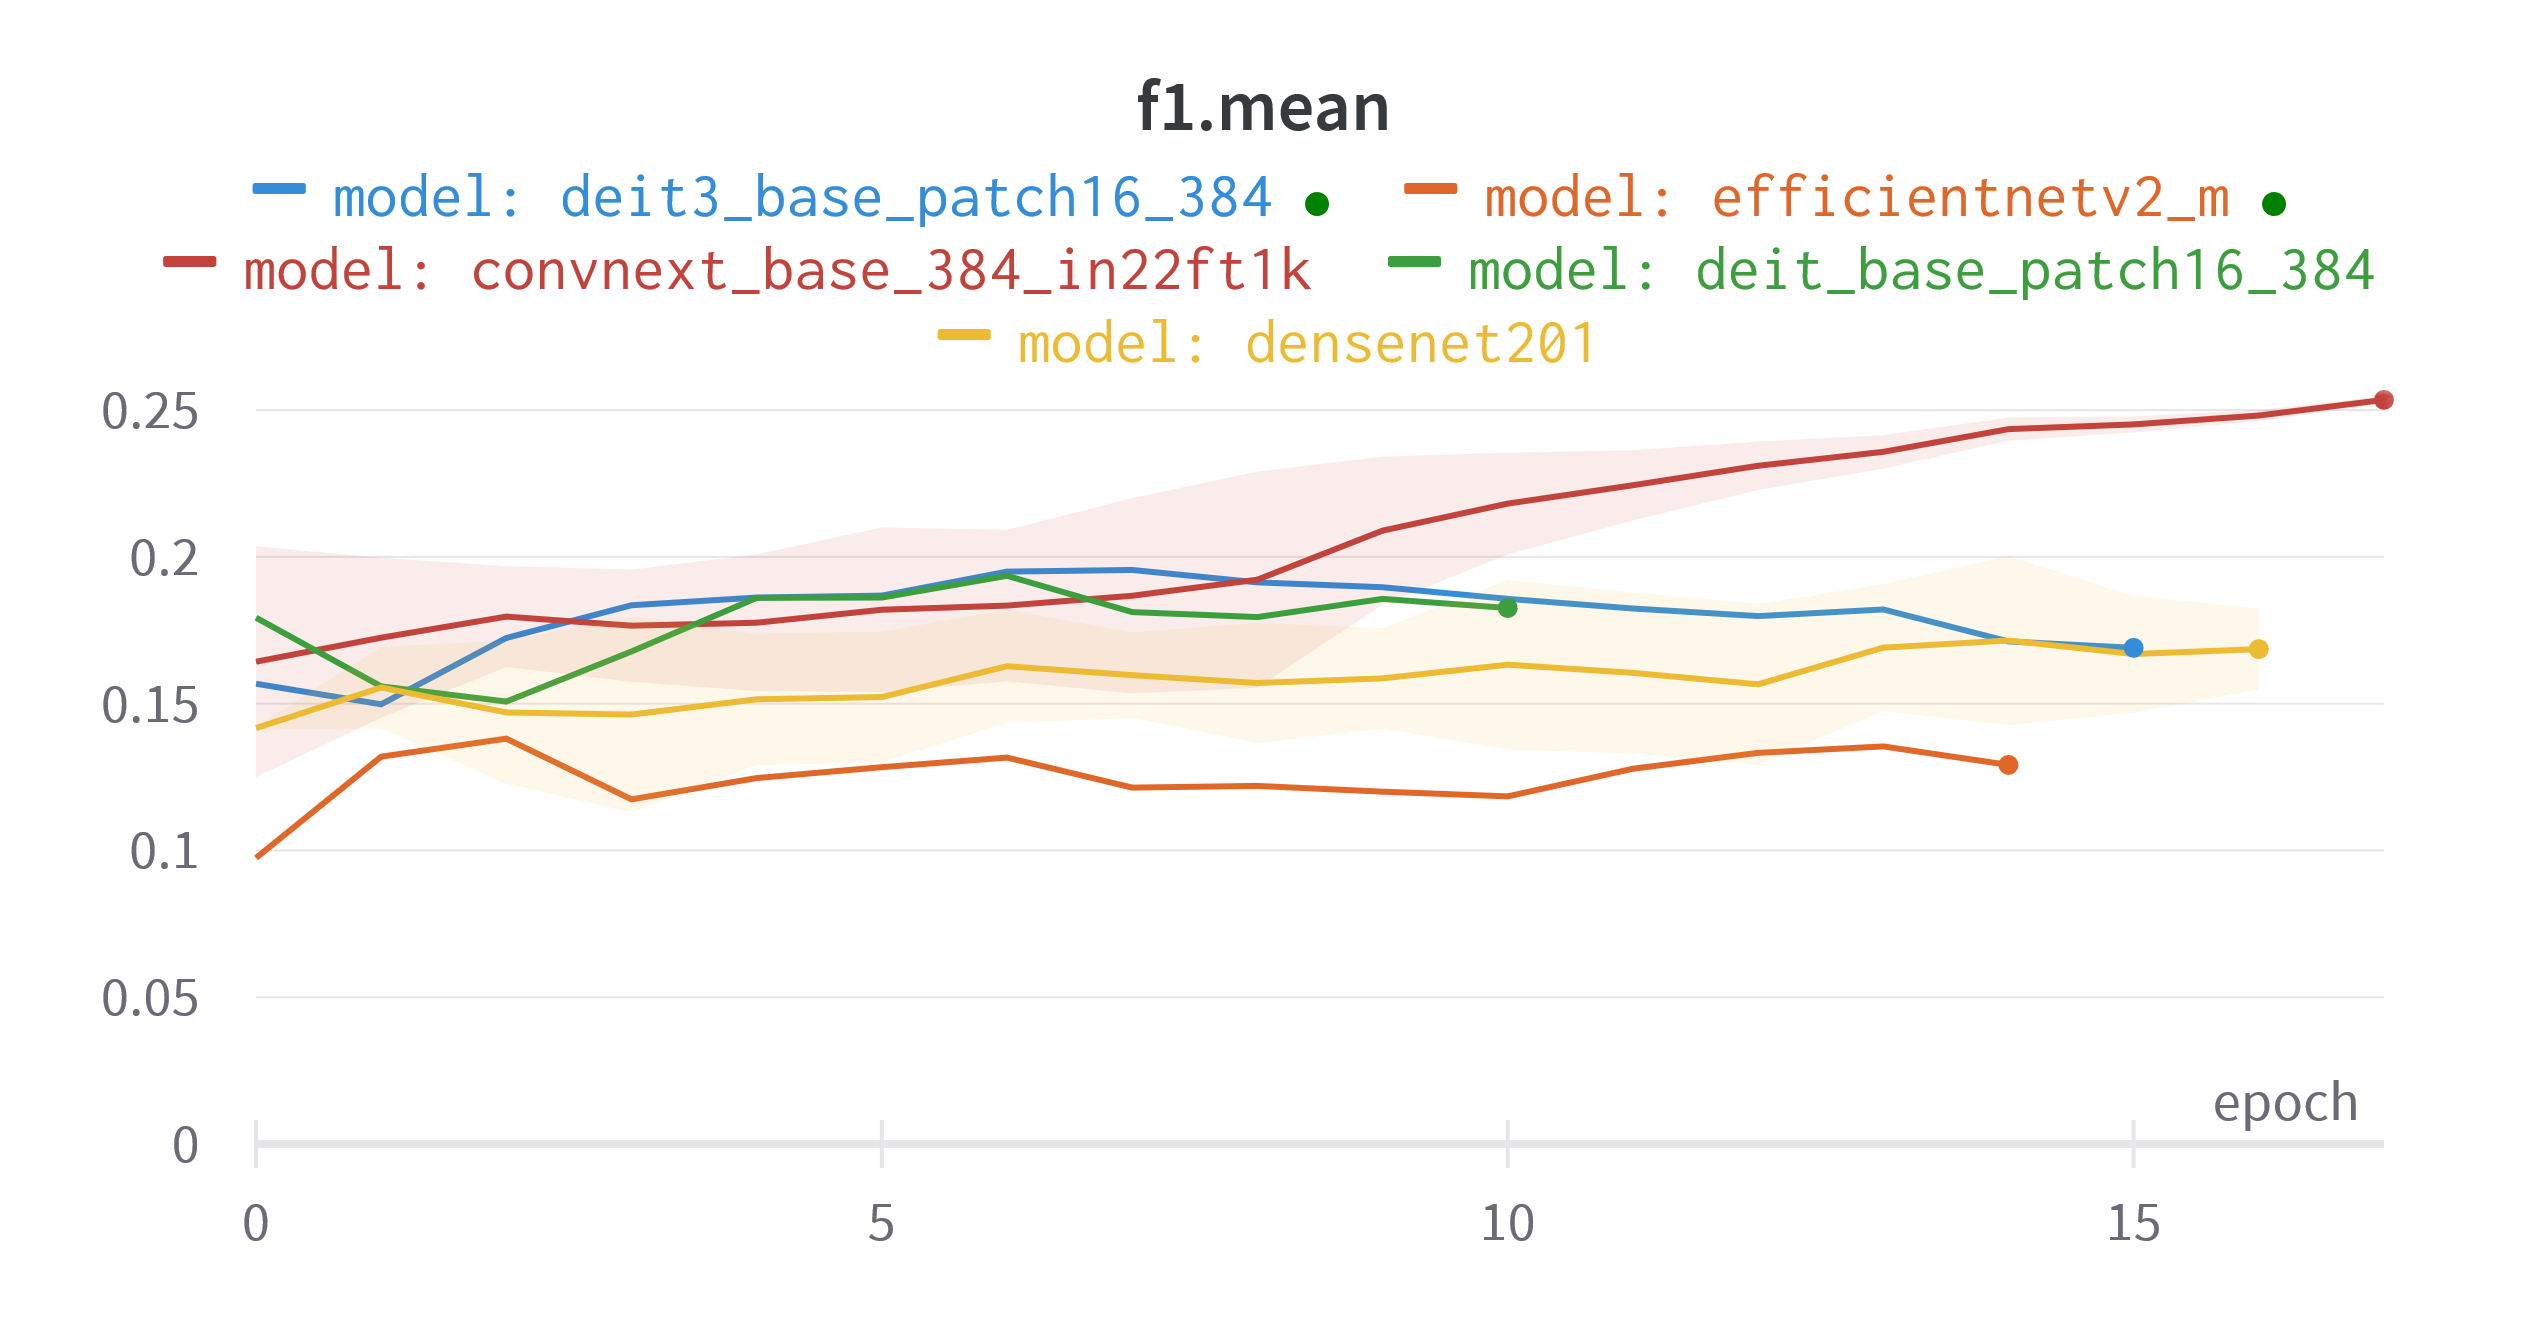
\includegraphics[width=\textwidth]{plots/model_comparison_f1}
                         \caption{Training loss}
                         \vspace{4ex}
                         \label{fig:model_comparison_f1}
                     \end{subfigure}
                     \hfill
                     \begin{subfigure}[b]{0.45\textwidth}
                         \centering
                         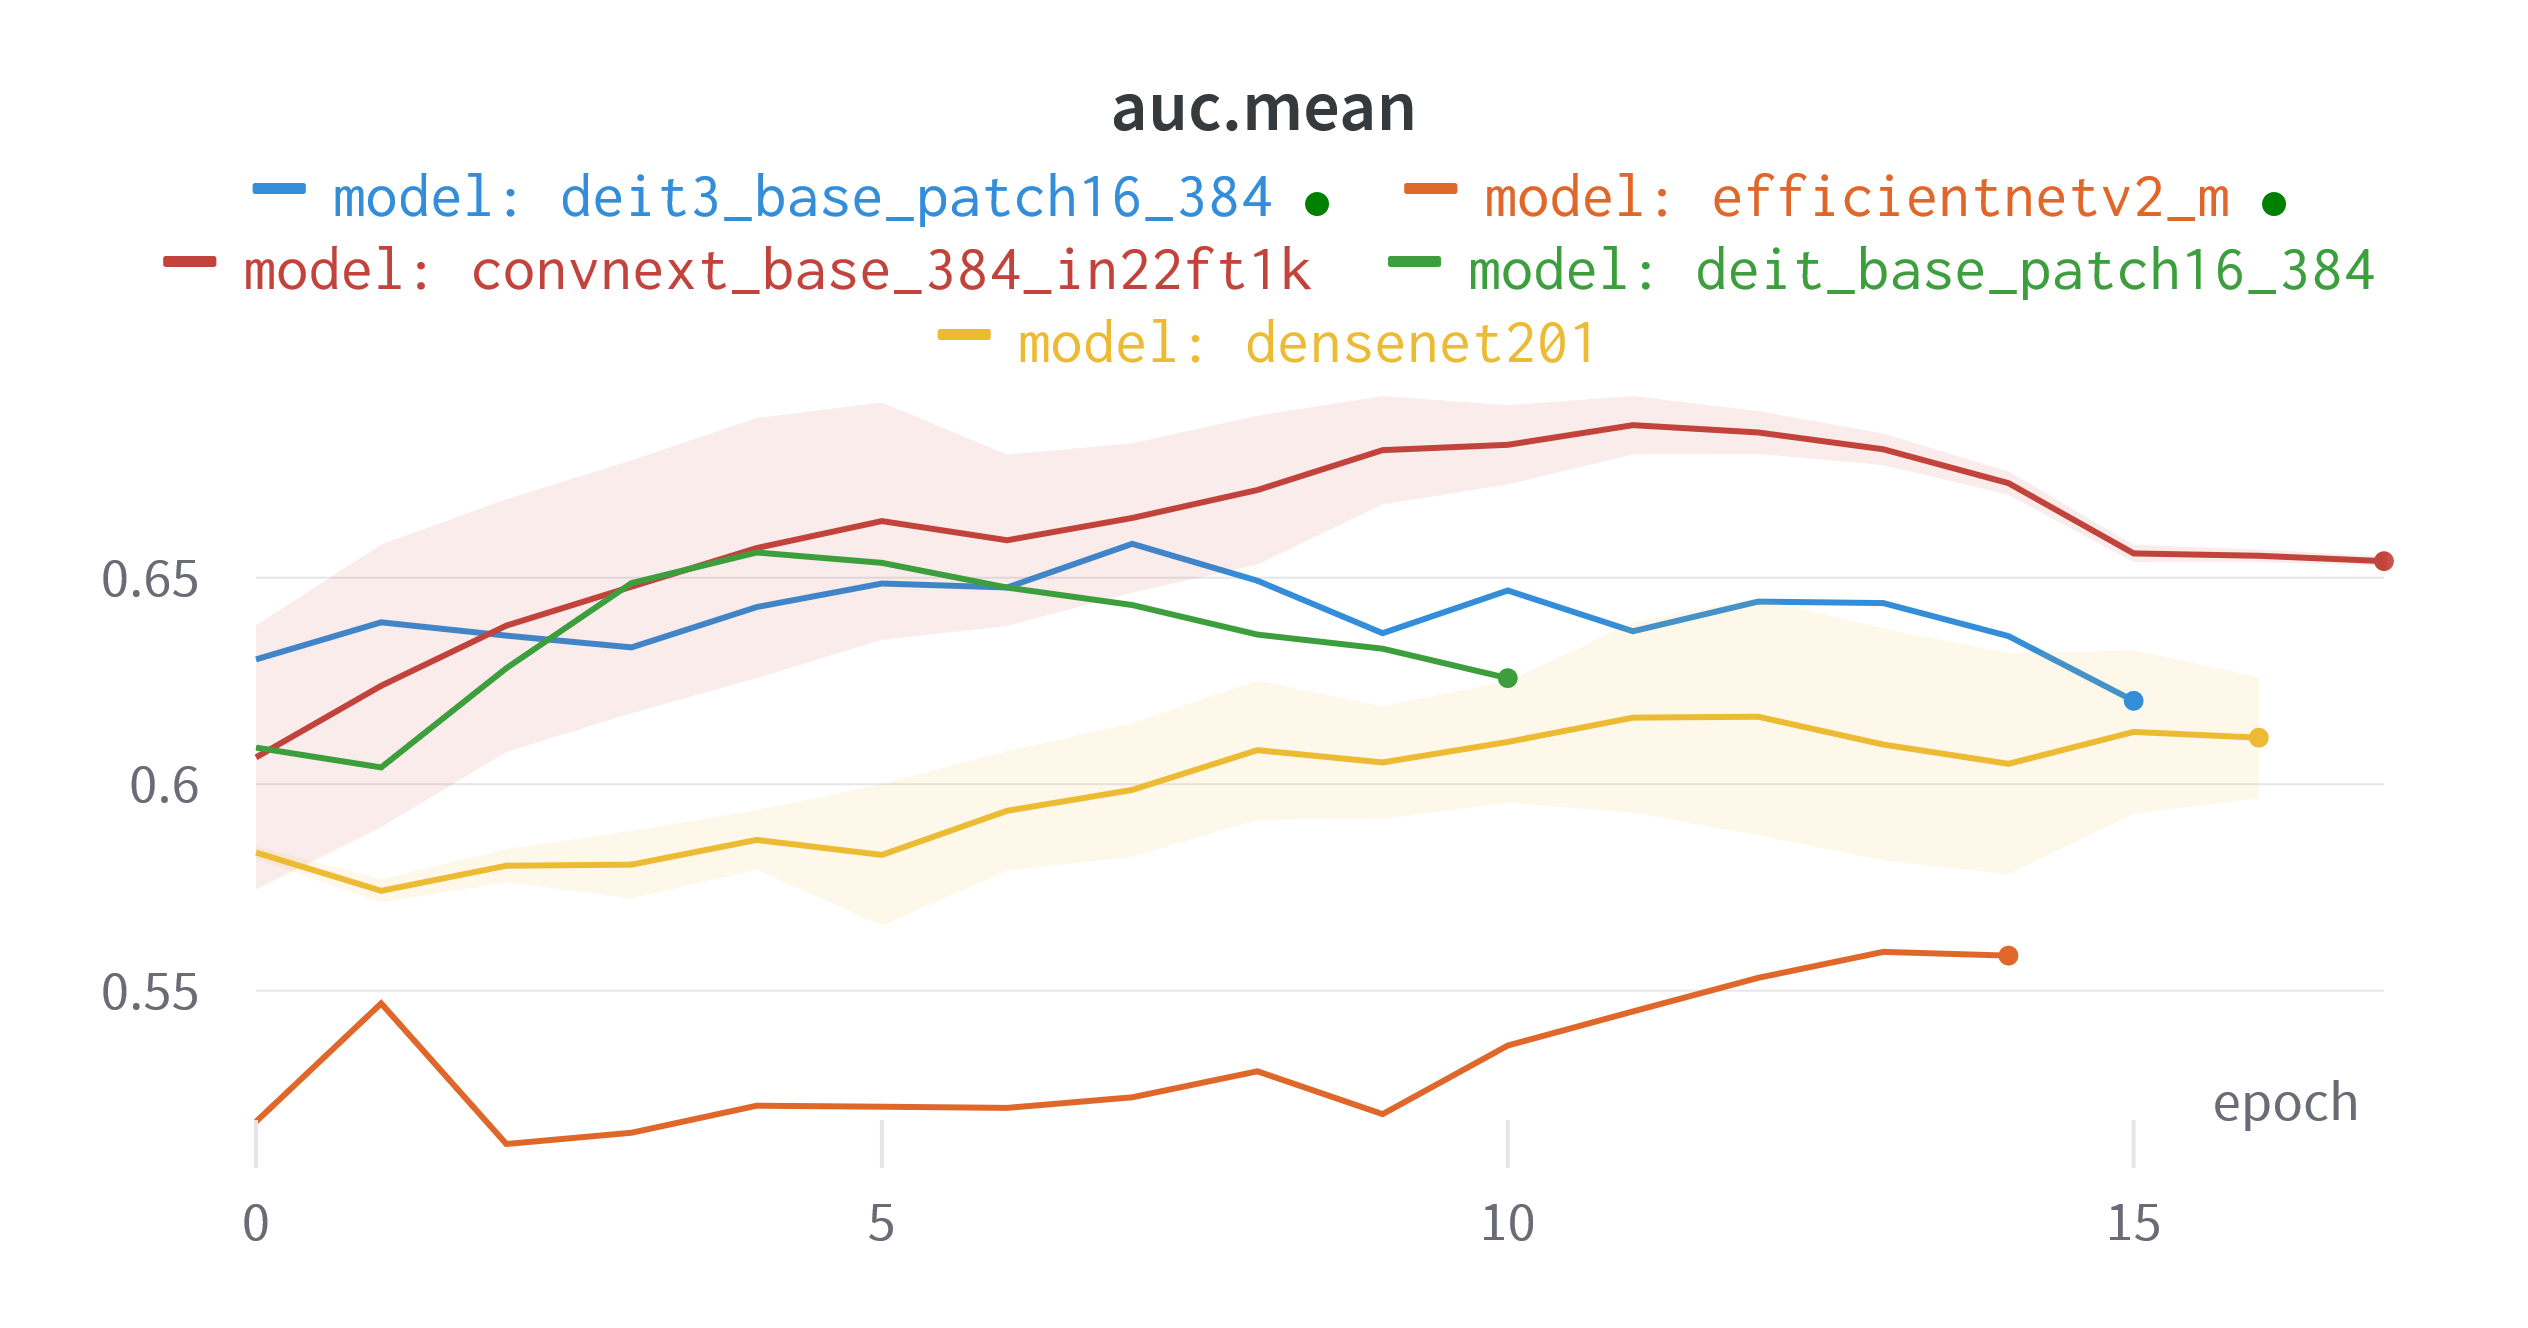
\includegraphics[width=\textwidth]{plots/model_comparison_auc}
                         \caption{Validation loss}
                         \vspace{4ex}
                         \label{fig:model_comparison_auc}
                     \end{subfigure}
                     \label{fig:model_comparison}
                     \caption{Comparisons of the experiments results grouped by model.The curve are smoothed out to help the analysis, and the error bars are the min-max
                         of the values.}
                \end{figure}


                \begin{figure}[H]
                     \centering
                     \begin{subfigure}[b]{0.45\textwidth}
                         \centering
                         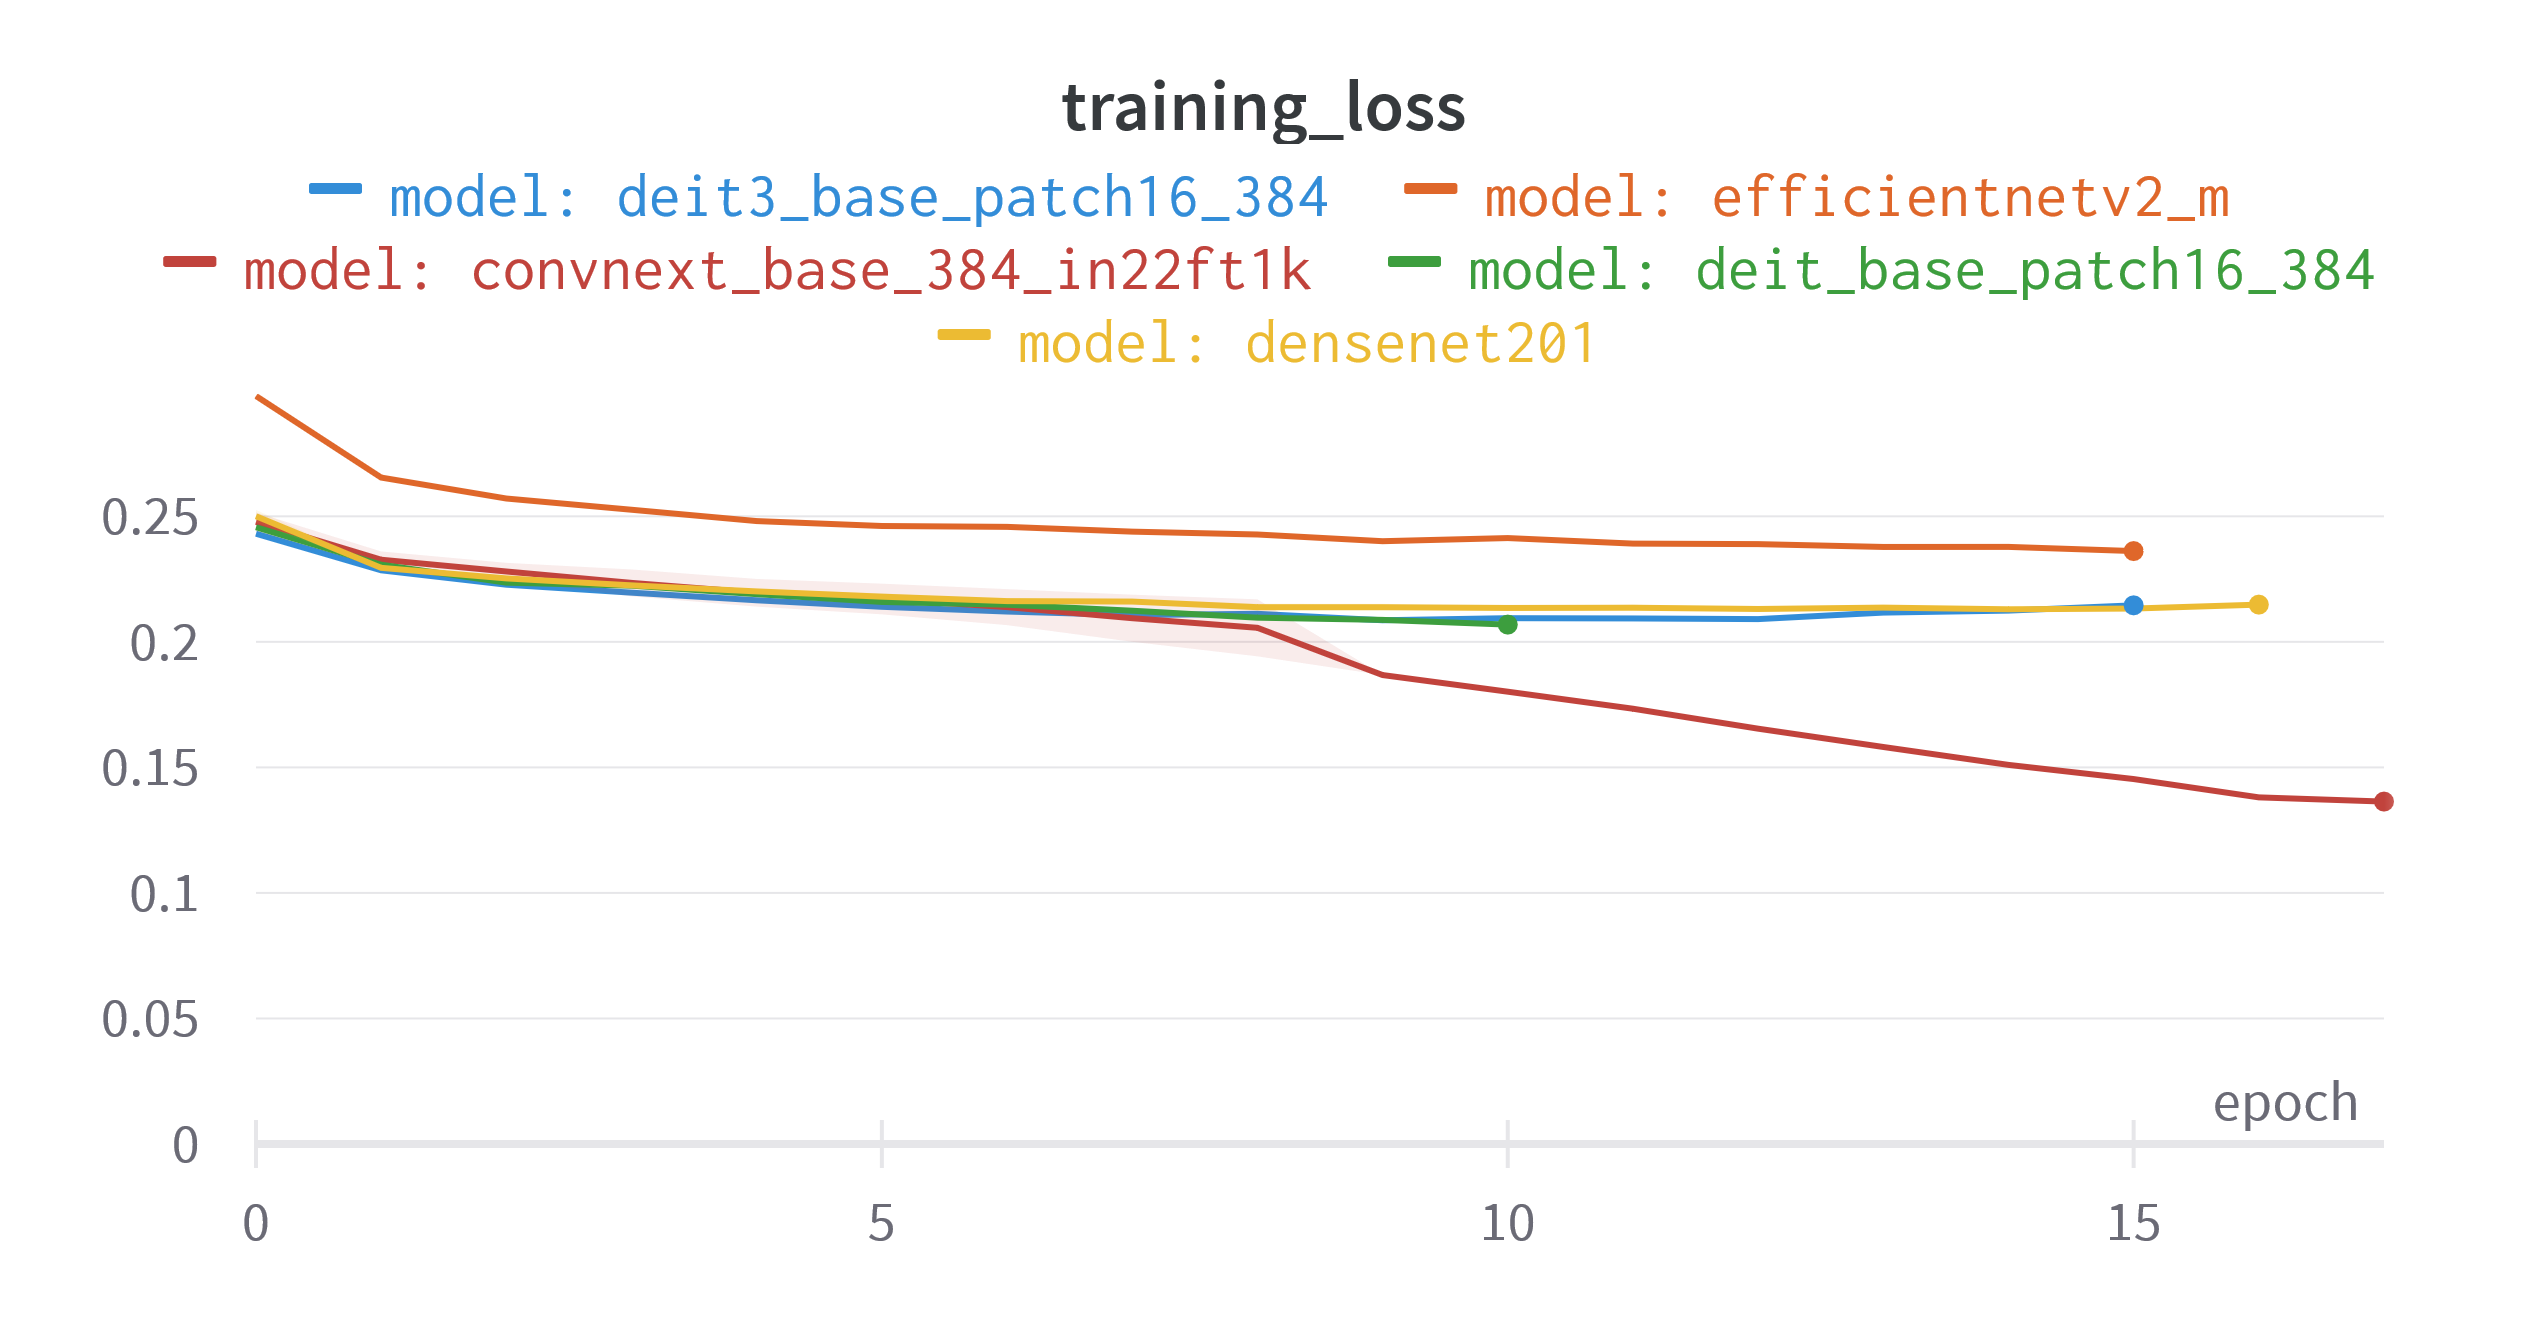
\includegraphics[width=\textwidth]{plots/chexpert_training_loss2}
                         \caption{Training loss}
                         \vspace{4ex}
                         \label{fig:chexpert_training_loss2}
                     \end{subfigure}
                     \hfill
                     \begin{subfigure}[b]{0.45\textwidth}
                         \centering
                         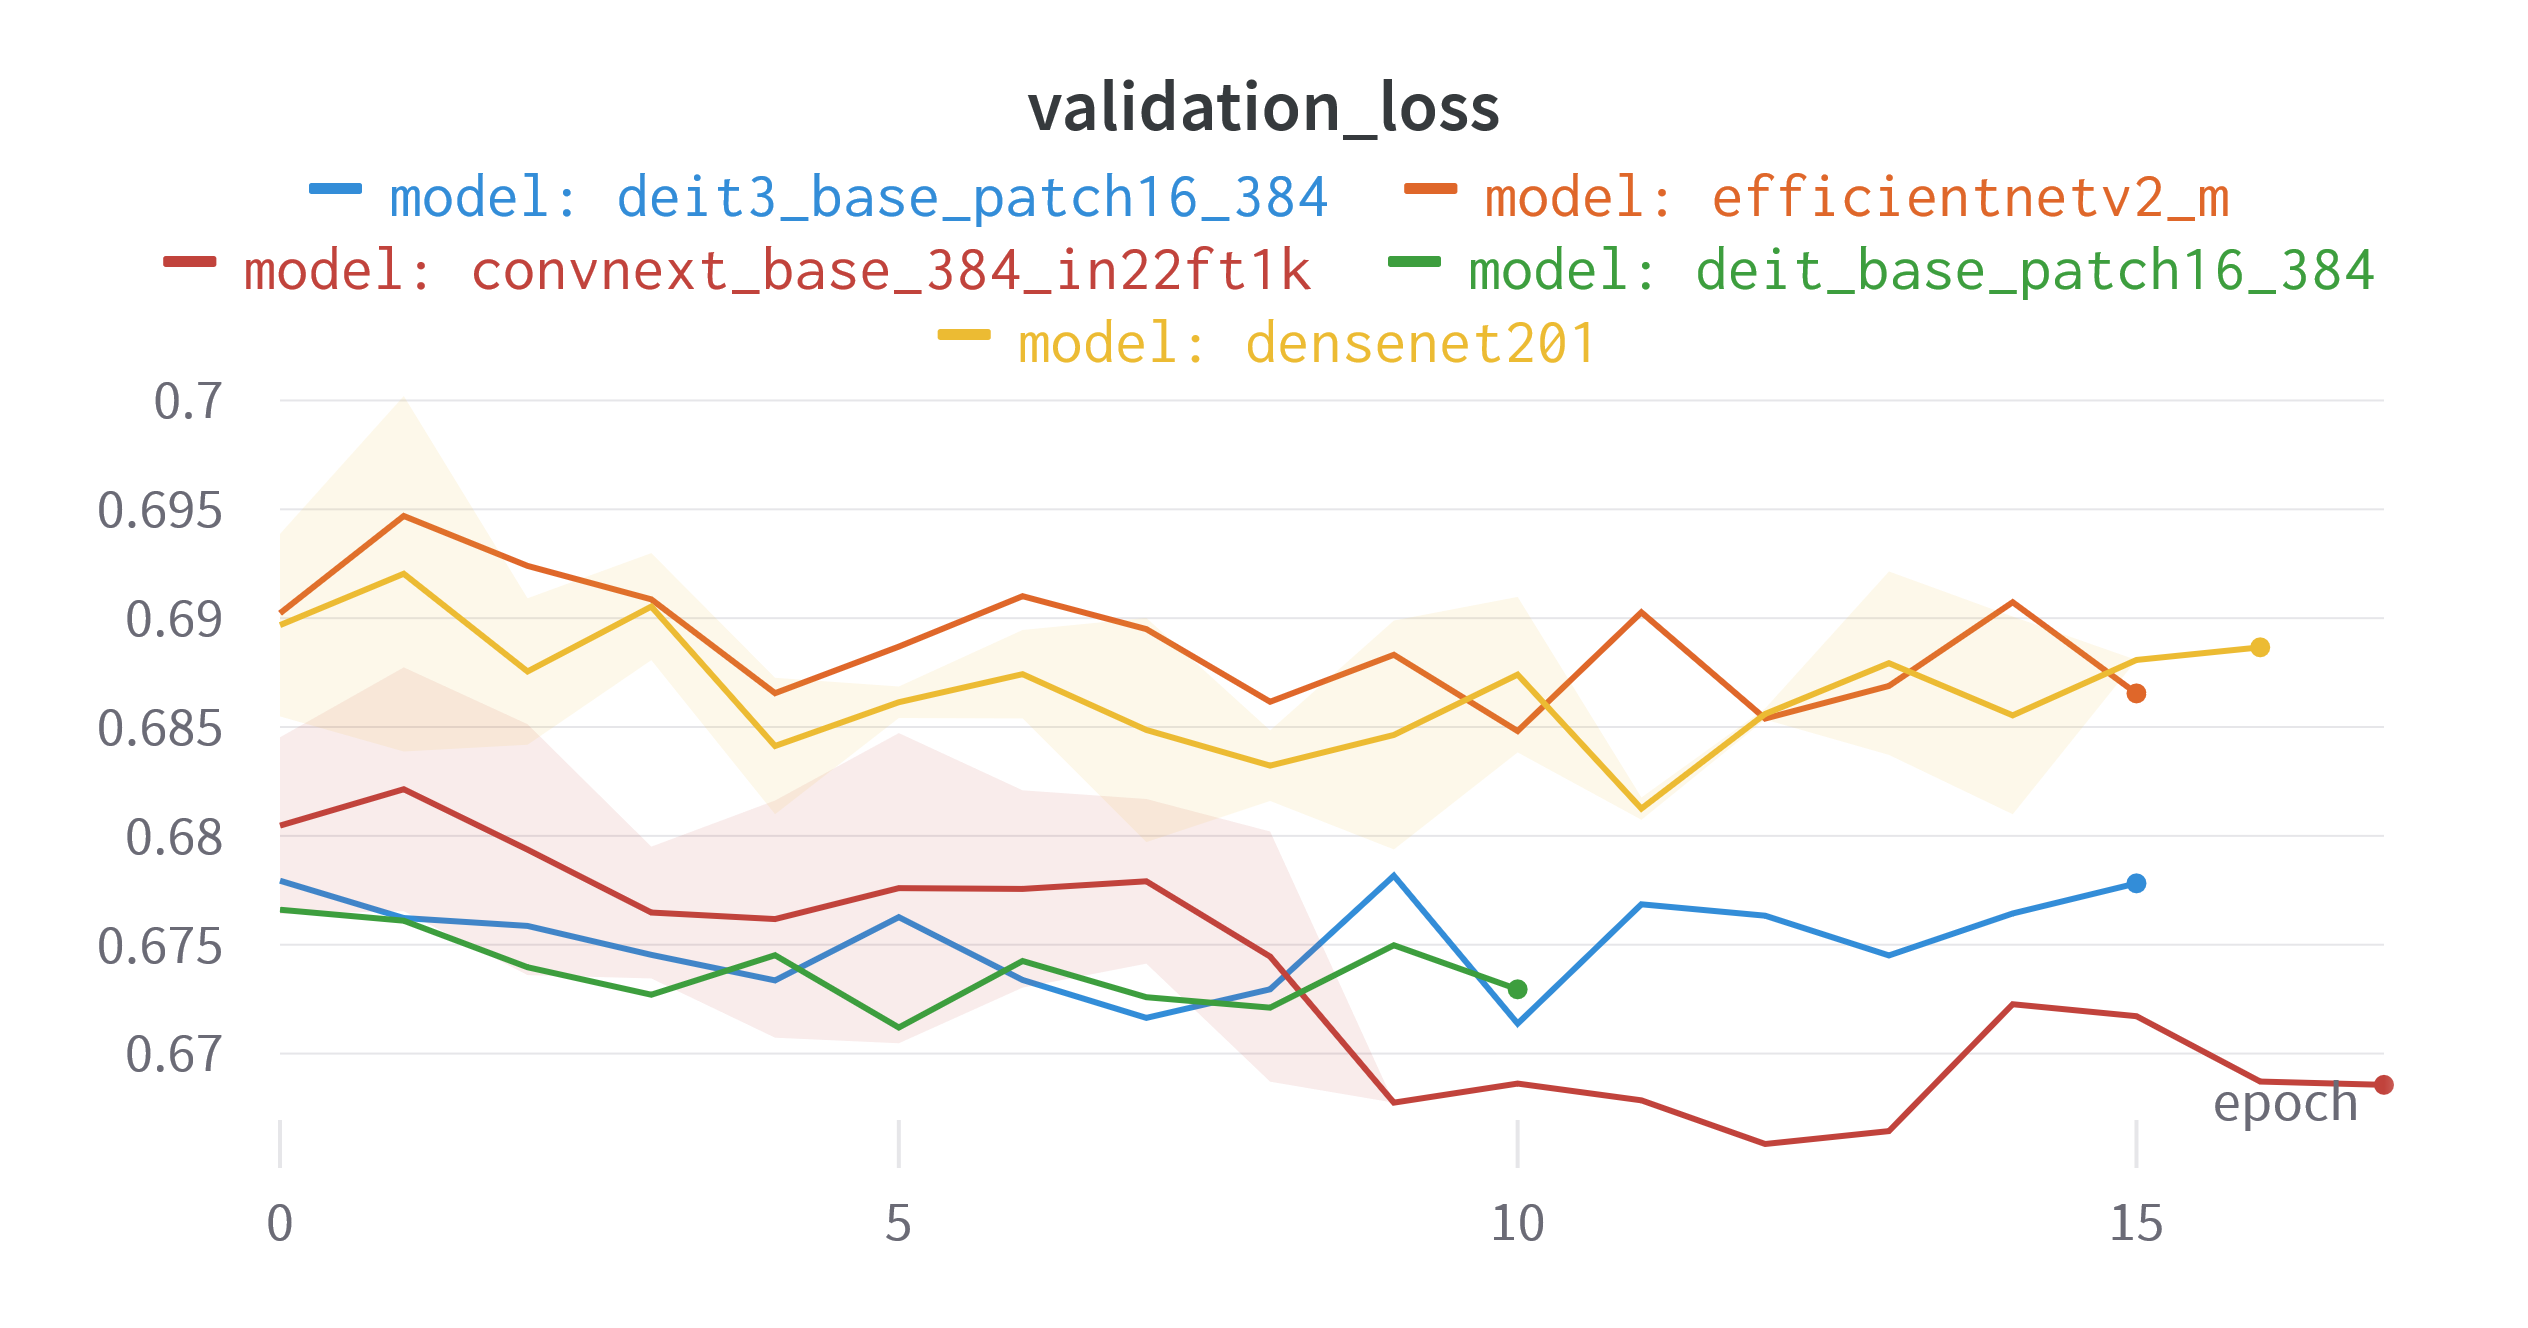
\includegraphics[width=\textwidth]{plots/chexpert_validation_loss2}
                         \caption{Validation loss}
                         \vspace{4ex}
                         \label{fig:chexpert_validation_loss2}
                     \end{subfigure}
                     \label{fig:training_curves2}
                     \caption{Training curves for oursecond attempt at reproducing the CheXpert baseline. The different runs are grouped by models.}
                \end{figure}



                We can now separate our results by the model choice to see which one is the best.As can be seen in
                the figure~\ref{fig:training_curves2} and~\ref{fig:model_comparison}, while the DenseNet model does
                learn from the data, it still underfit while the convnext model is able to overfit our training data.
                This does seem to indicate that we need a more complex model than the densenet.
                However, the convnext model is able to achieve a better AUC than Densenet. It means that while by itself, the training curves seem
                to indicate an overfitting, since our f1 is still increasing, our model is learning to classify better. This means the difference in loss in between the training
                and validation set is seemingly due to the difference in distribution of the two.

                For our next experiment, we should therefore continue with the ConvNeXt model, and increase the data
                augmentation. Depending on those results, we can later try to add different data augmentations
                technique or a larger version of the ConvNeXt model.

                We can also consider to use the positive weight depending on whether we prefer optimizing the AUC or the F1-score. Future discussions with the radiologist
                that will be using our model will help us decide which metric is the most important. In the meantime, I think it would be best to improve the F1-score as
                it is the metric that is most similar to the radiologist's estimation. It will be more intuitive to have a model that has a threshold at 0.5, and that express
                some uncertainty when the probability is between 0.4 and 0.6. This is not the case with the AUC, as it is a metric that gains points for being very close to 0 or 1.

                Finally, we can see that while the validation loss is a bit chaotic, the training loss decrease while the f1-score is still increasing. This indicate
                that the model is still learning from the data. We should therefore continue to train the model for a few more epochs. To do that, we should therefore increase the patience
                to 10 or 20 epochs.


                Just as we compared the performance by the choice of model, we can do the same to compare the performance of using 1 vs 3 channels. Doing so, we can observe
                in the figure~\ref{fig:channel_comparison} that the model with 3 channels is able to achieve a better AUC and F1-score. This is most likely due to the fact that the model is able to
                extract more information as we did not simply reapeated the same information on the three channel, but instead concatenated the min-max normalized image, and two image treated
                with the CLAHE algorithm, albeit with two different threshold (2 and 4). But while it performs slightly better, it is not by a large margin, but it does increase the training time significantly
                by putting a heavier load on the CPU. This is why we will continue to use the 1 channel model for the rest of the experiments, until we reach our final results.

            \subsubsection{Third Attempt}
            % Applying the lesson learned
            Applying the lesson learned, I tested the convnext base model with the 1 channels, and with/without the positive weights. I also increased the patience to 20 epochs.
            The results are shown in the figure~\ref{fig:training_curves3} and~\ref{fig:chexpert_results3}. We can see that the model with the positive weights is able to achieve a better AUC and F1-score.

            \begin{figure}[H]
                 \centering
                 \begin{subfigure}[b]{0.45\textwidth}
                     \centering
                     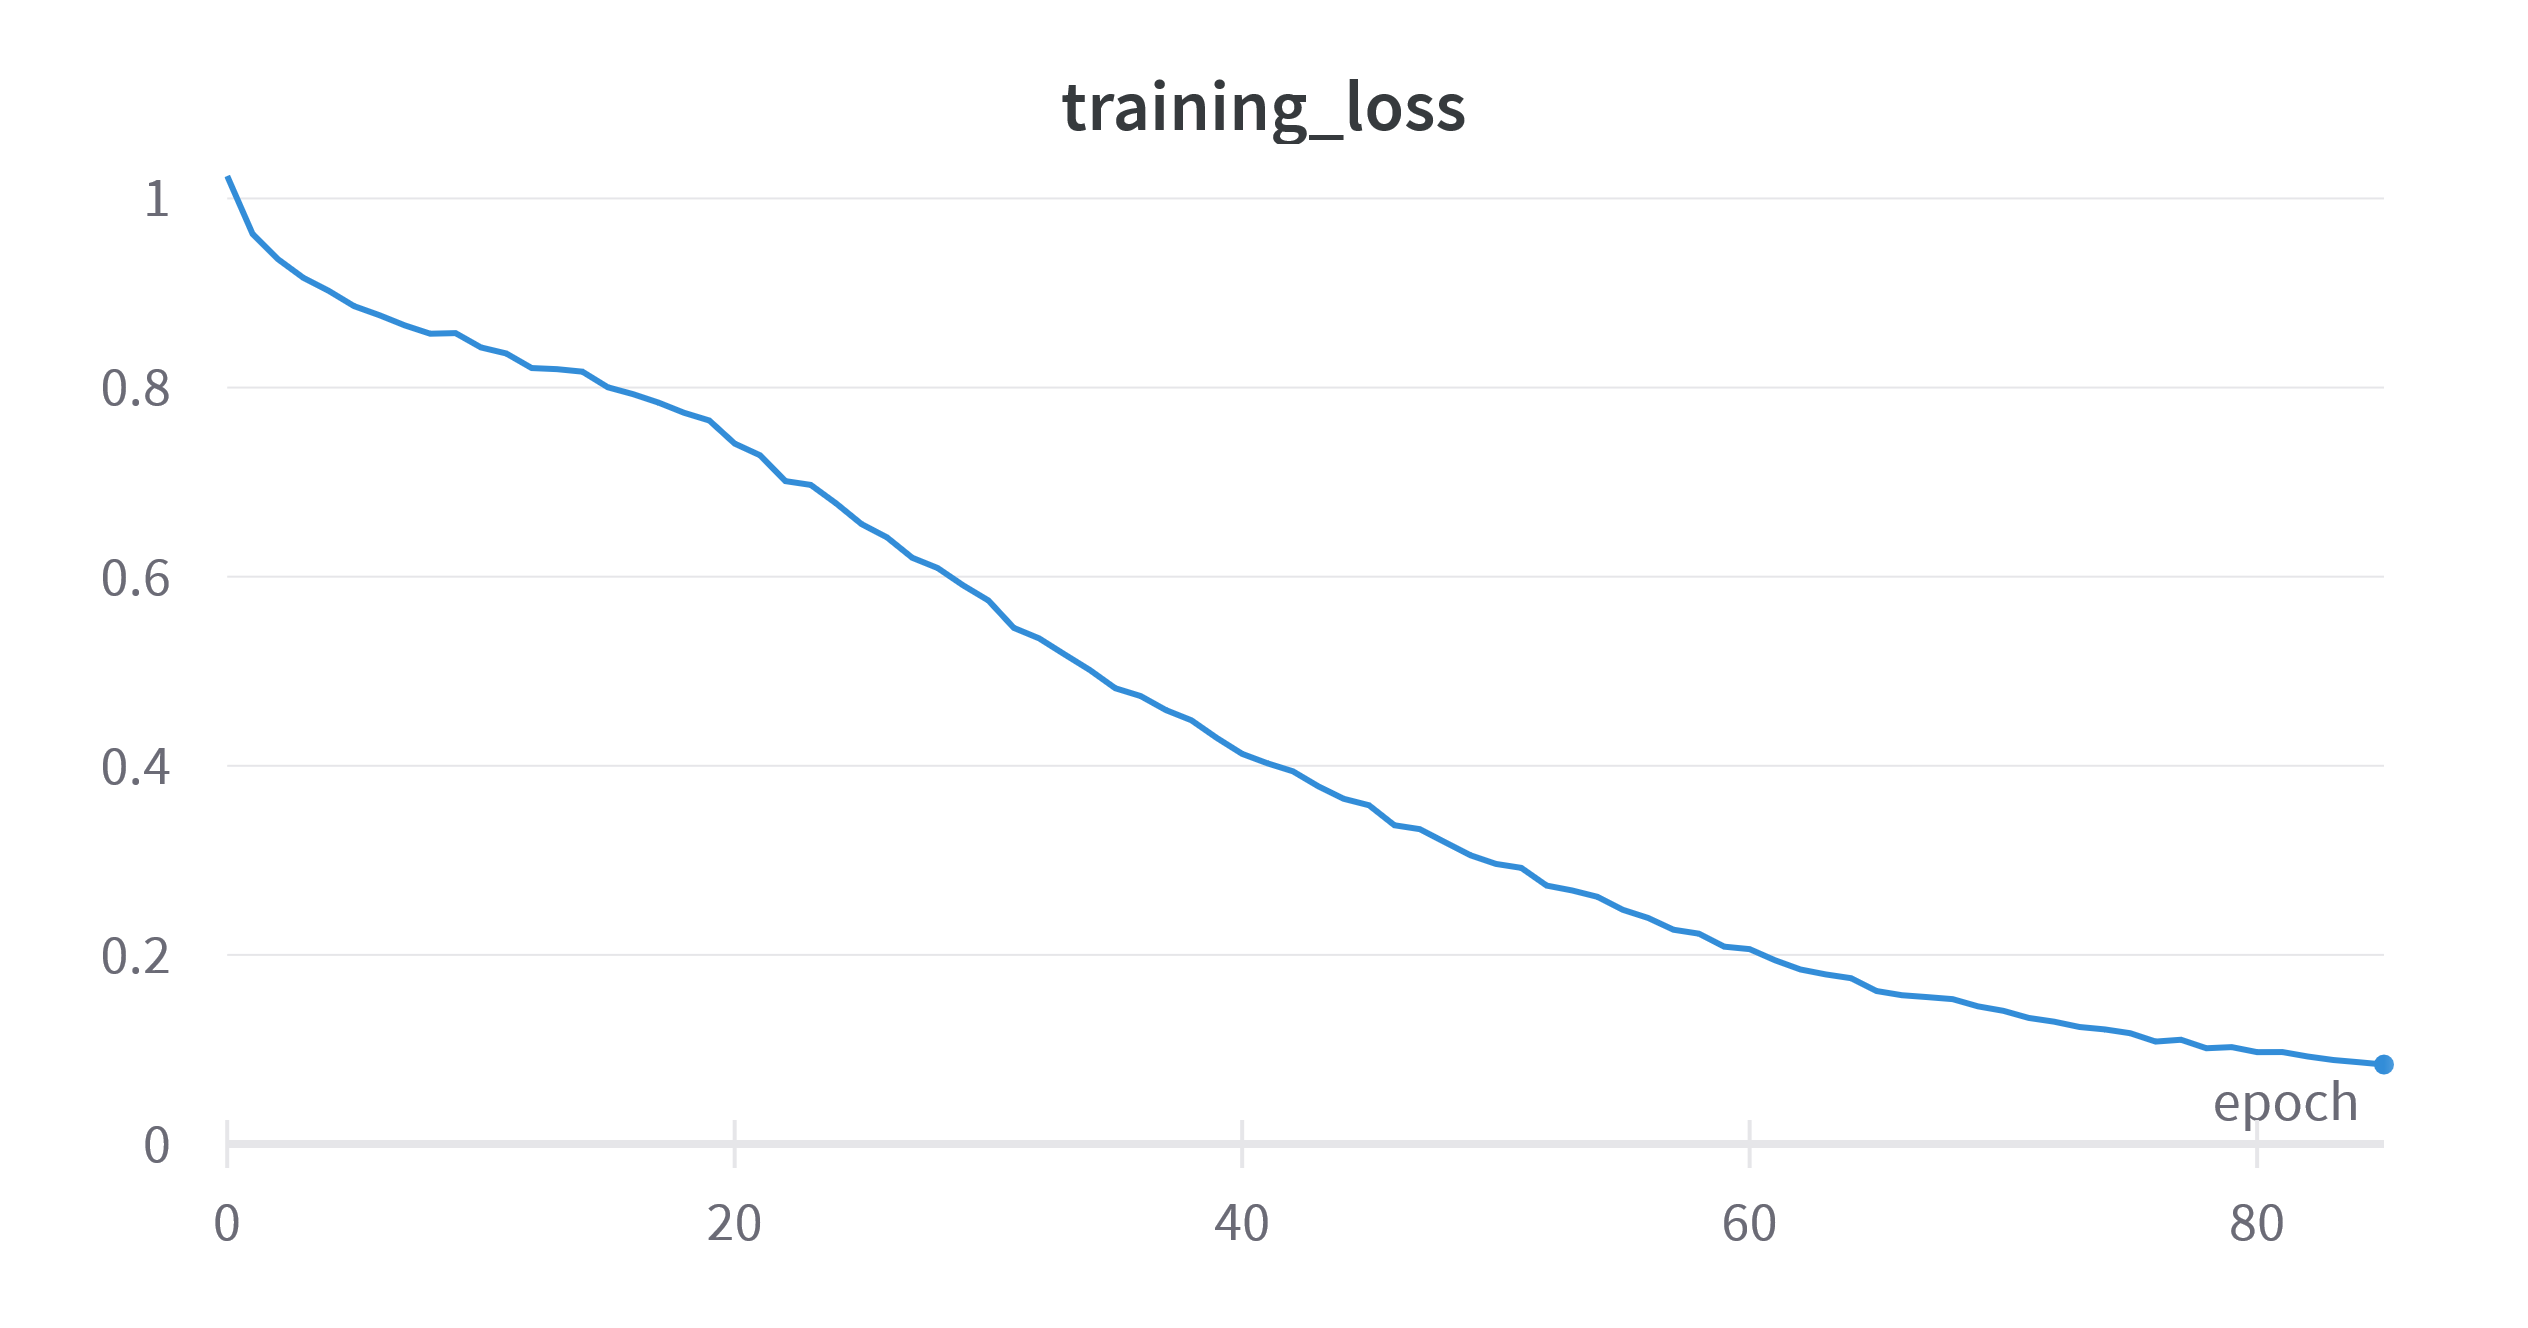
\includegraphics[width=\textwidth]{plots/chexpert_training_loss3}
                     \caption{Training loss}
                     \vspace{4ex}
                     \label{fig:chexpert_training_loss3}
                 \end{subfigure}
                 \hfill
                 \begin{subfigure}[b]{0.45\textwidth}
                     \centering
                     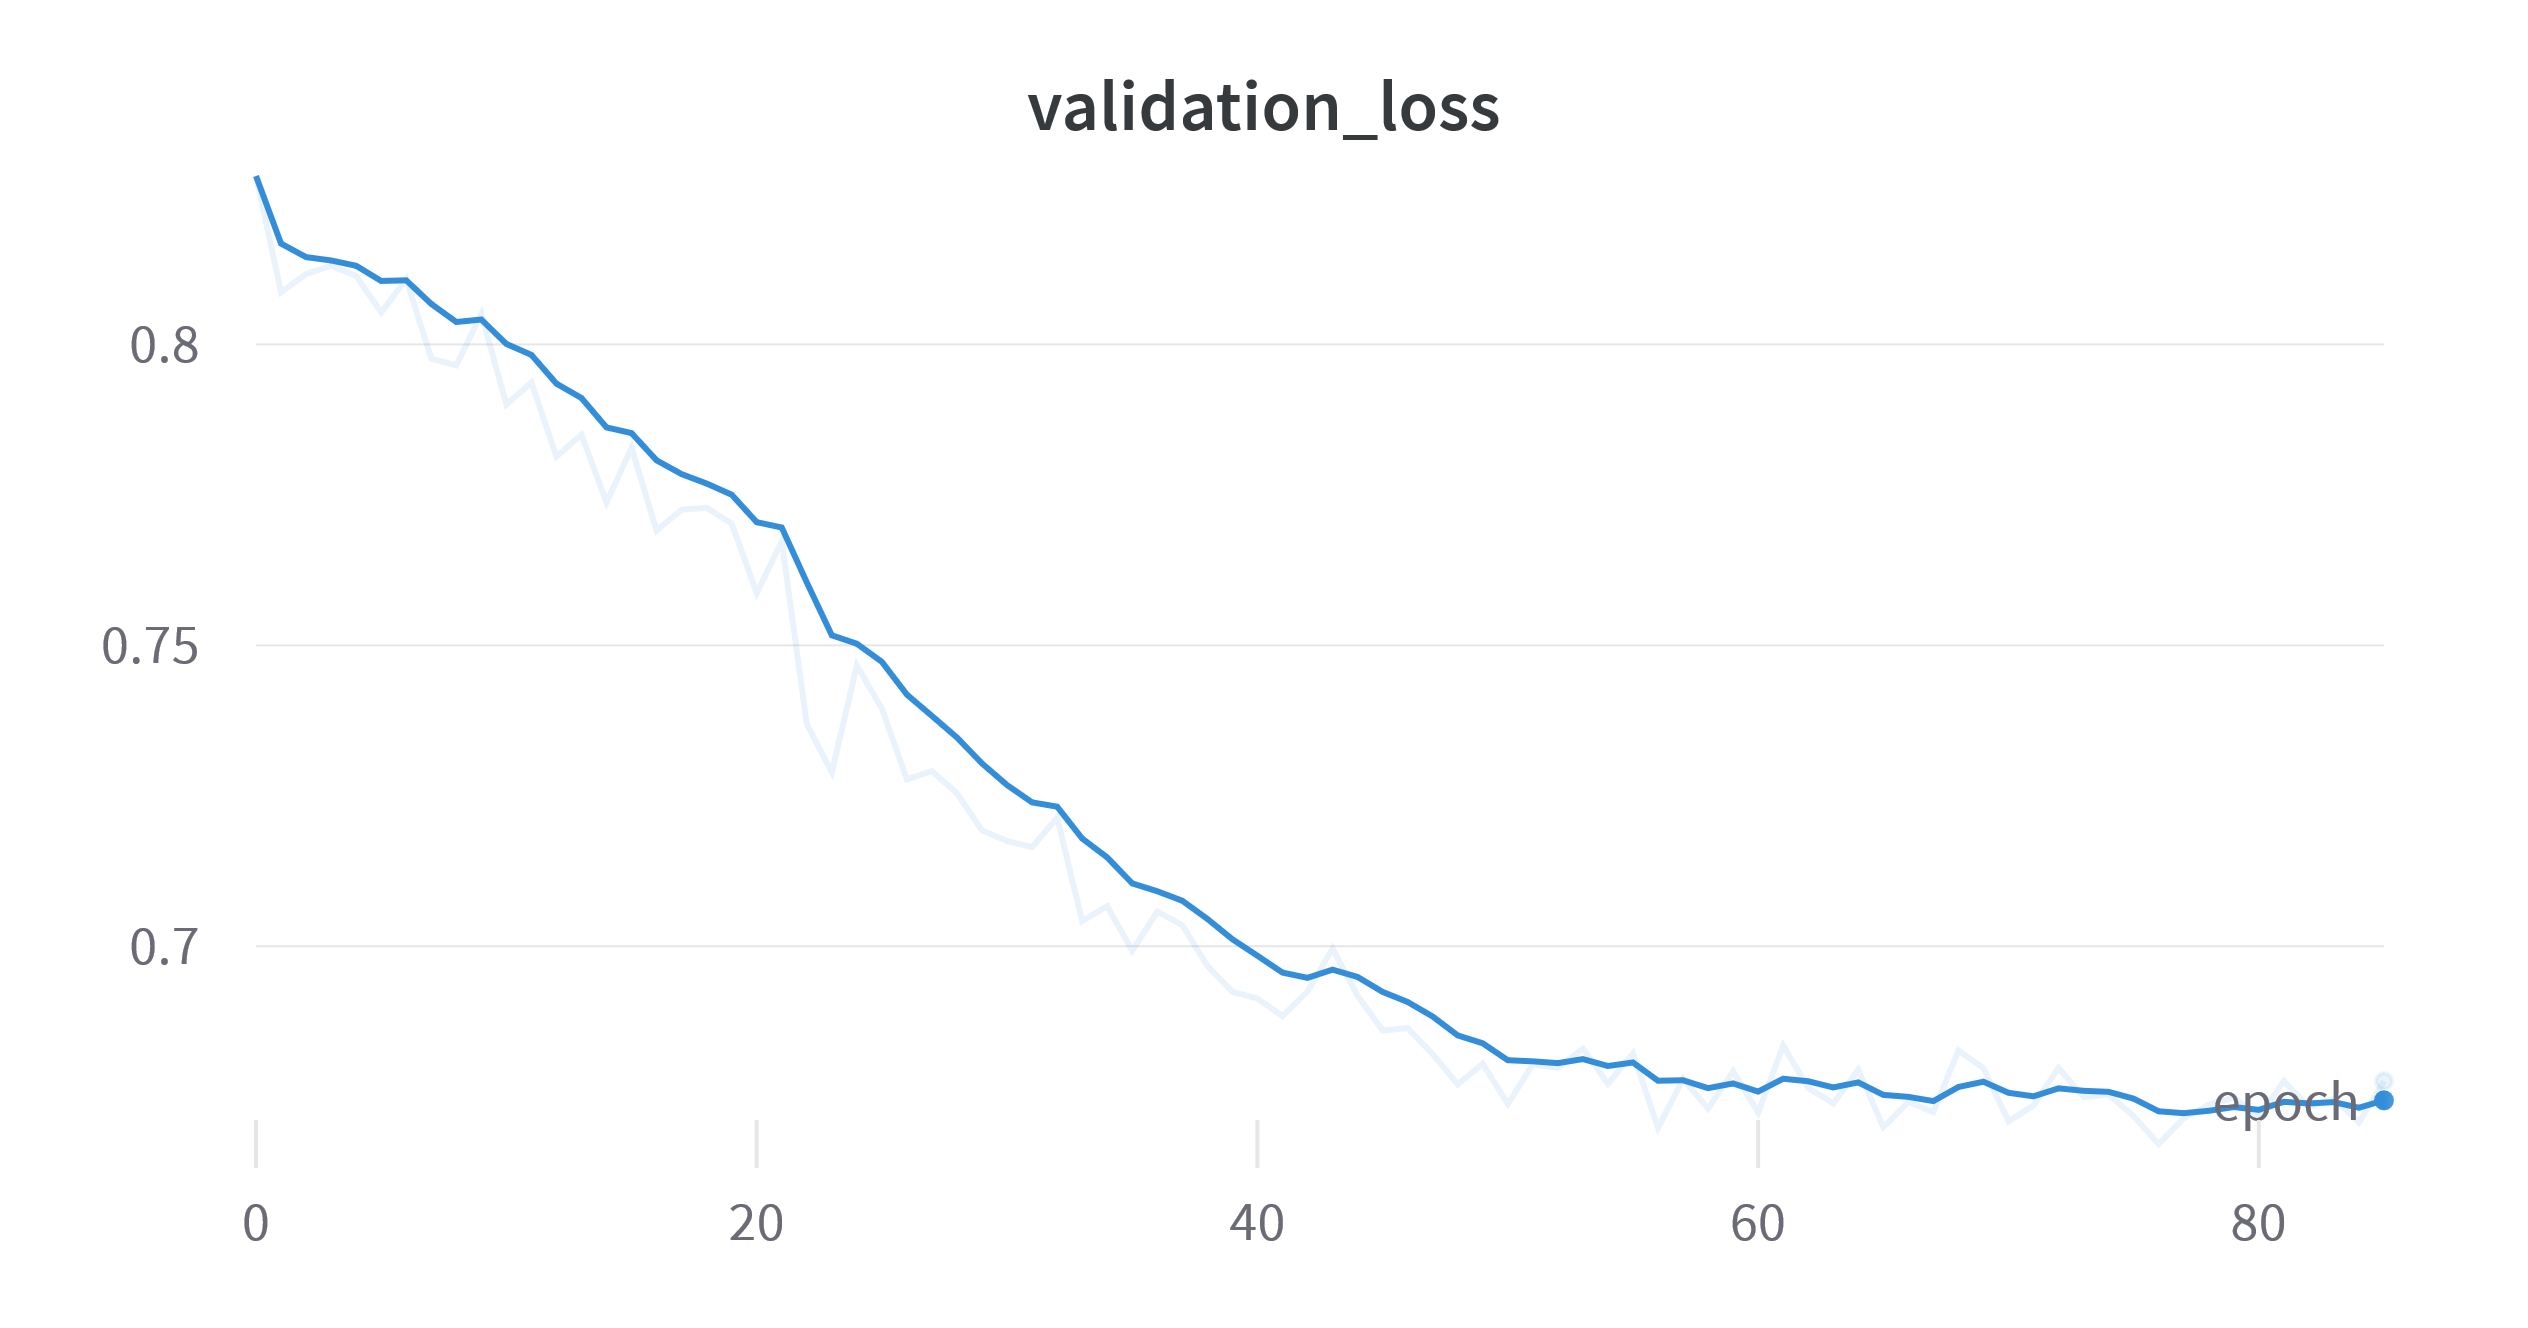
\includegraphics[width=\textwidth]{plots/chexpert_validation_loss3}
                     \caption{Validation loss}
                     \vspace{4ex}
                     \label{fig:chexpert_validation_loss3}
                 \end{subfigure}
                 \label{fig:training_curves3}
                 \caption{Training curves for our third attempt at reproducing the CheXpert baseline}

            \end{figure}

            \begin{figure}[H]
                 \centering
                 \begin{subfigure}[b]{0.45\textwidth}
                     \centering
                     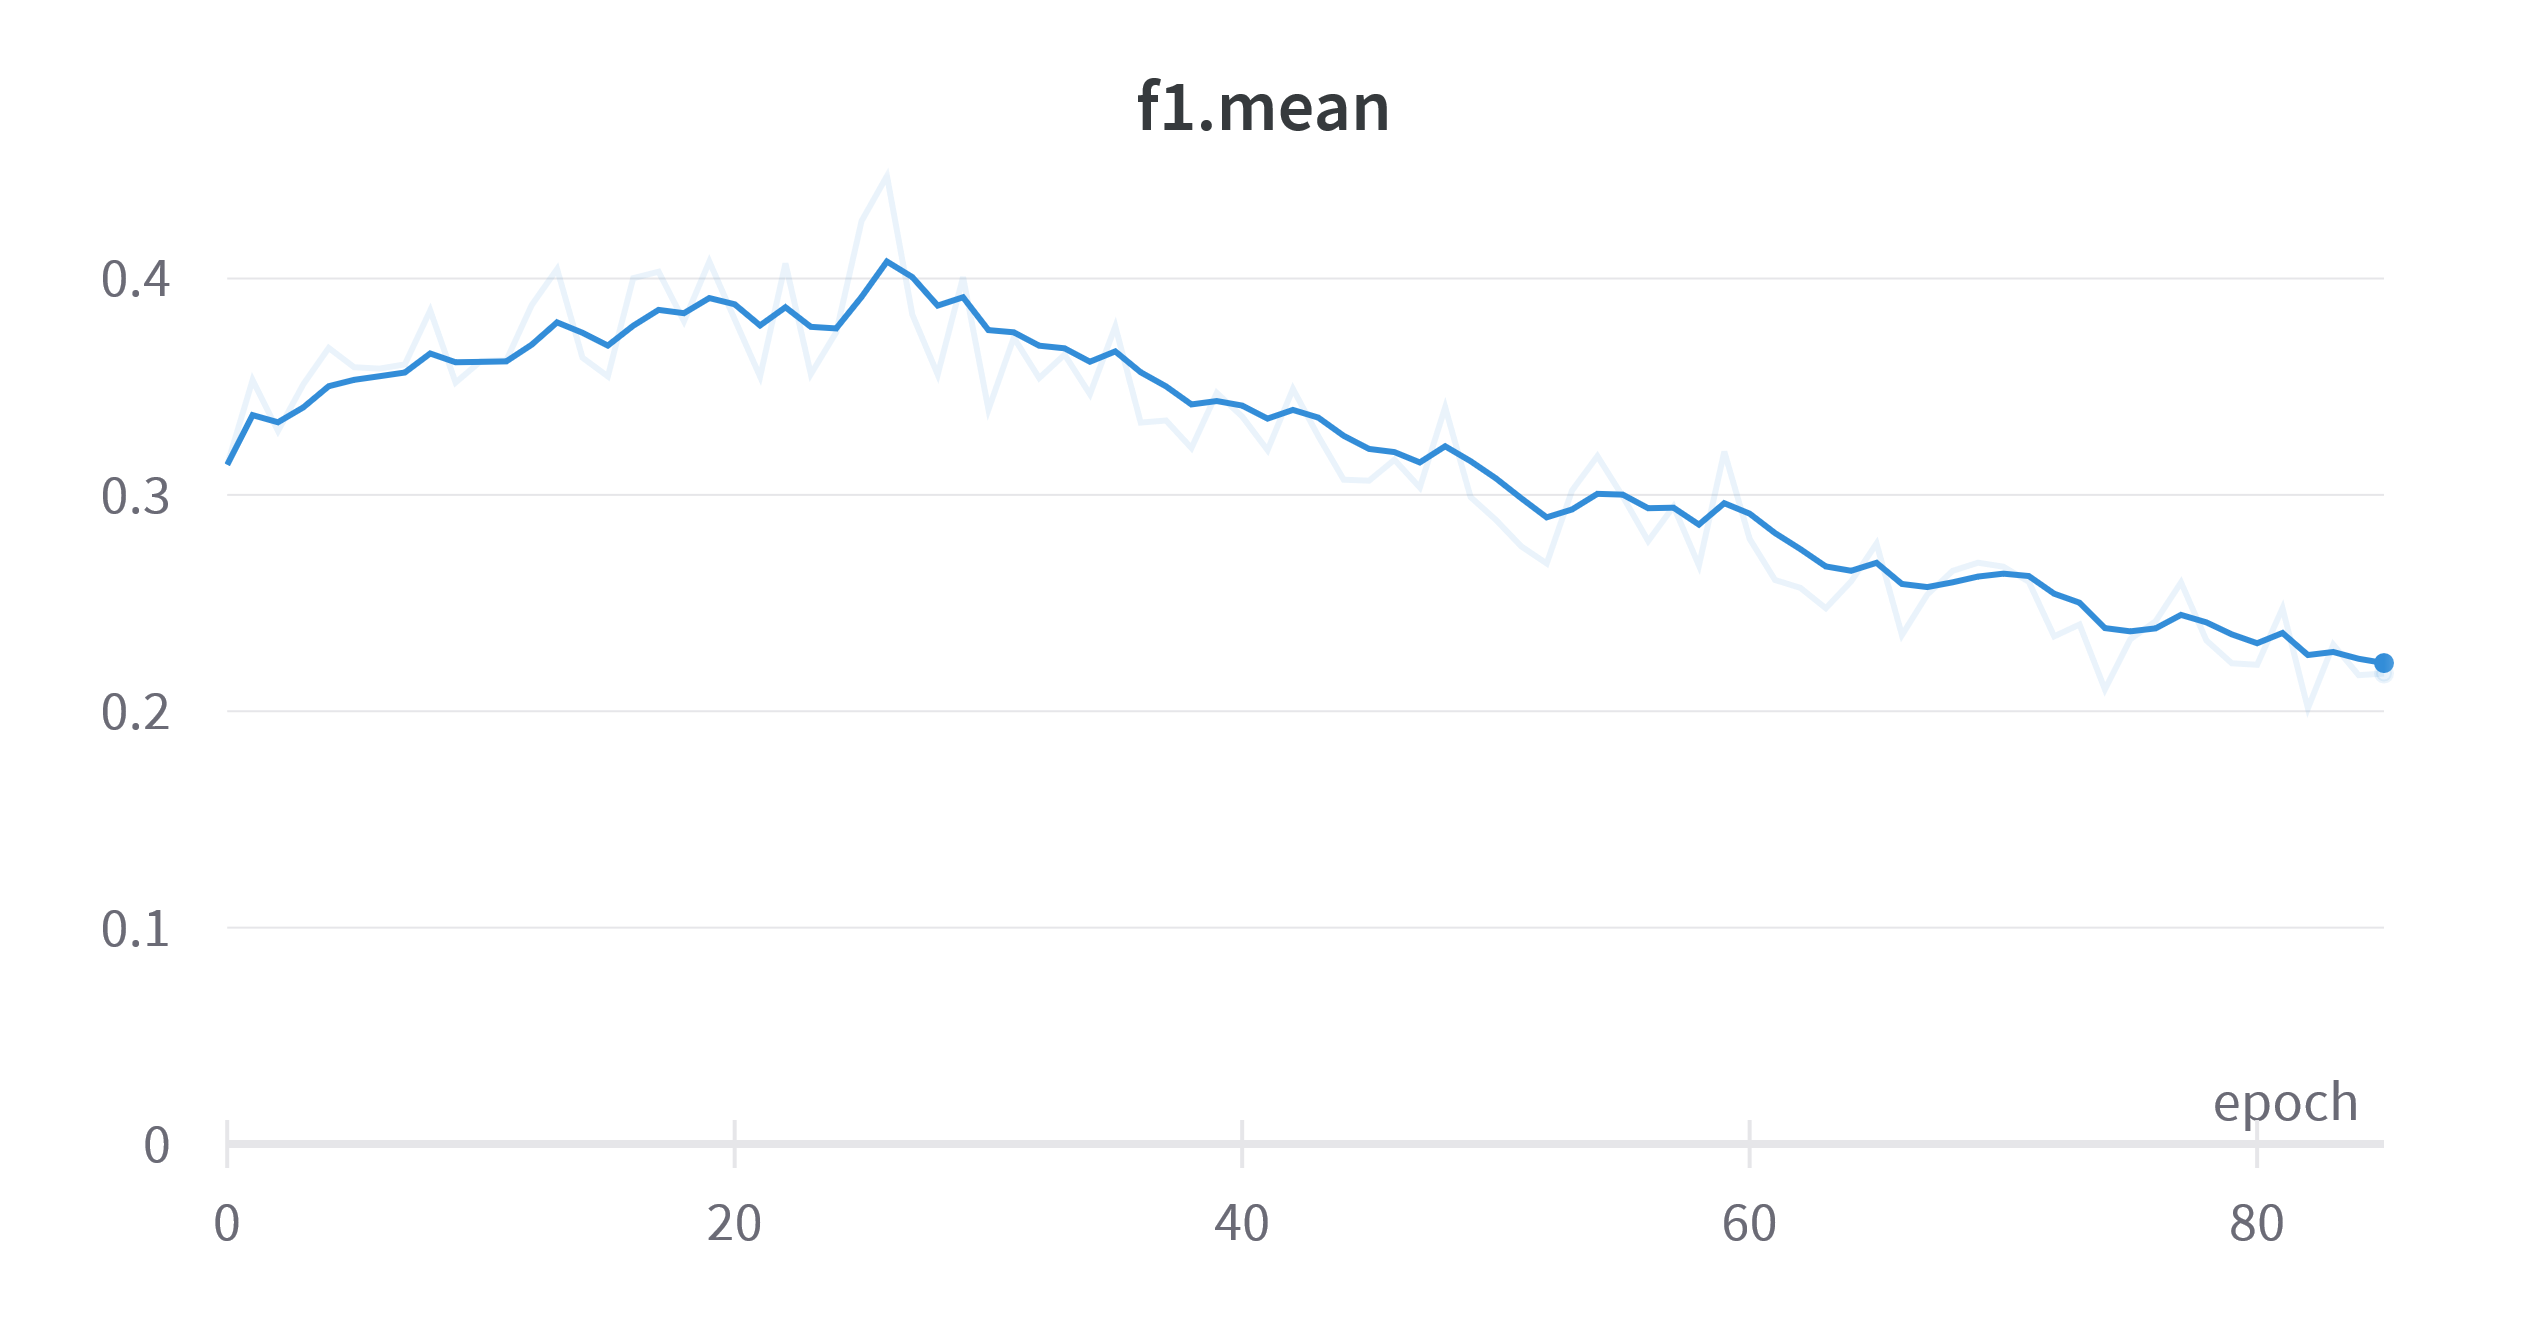
\includegraphics[width=\textwidth]{plots/chexpert_f1_3}
                     \caption{Training loss}
                     \vspace{4ex}
                     \label{fig:chexpert_f1_3}
                 \end{subfigure}
                 \hfill
                 \begin{subfigure}[b]{0.45\textwidth}
                     \centering
                     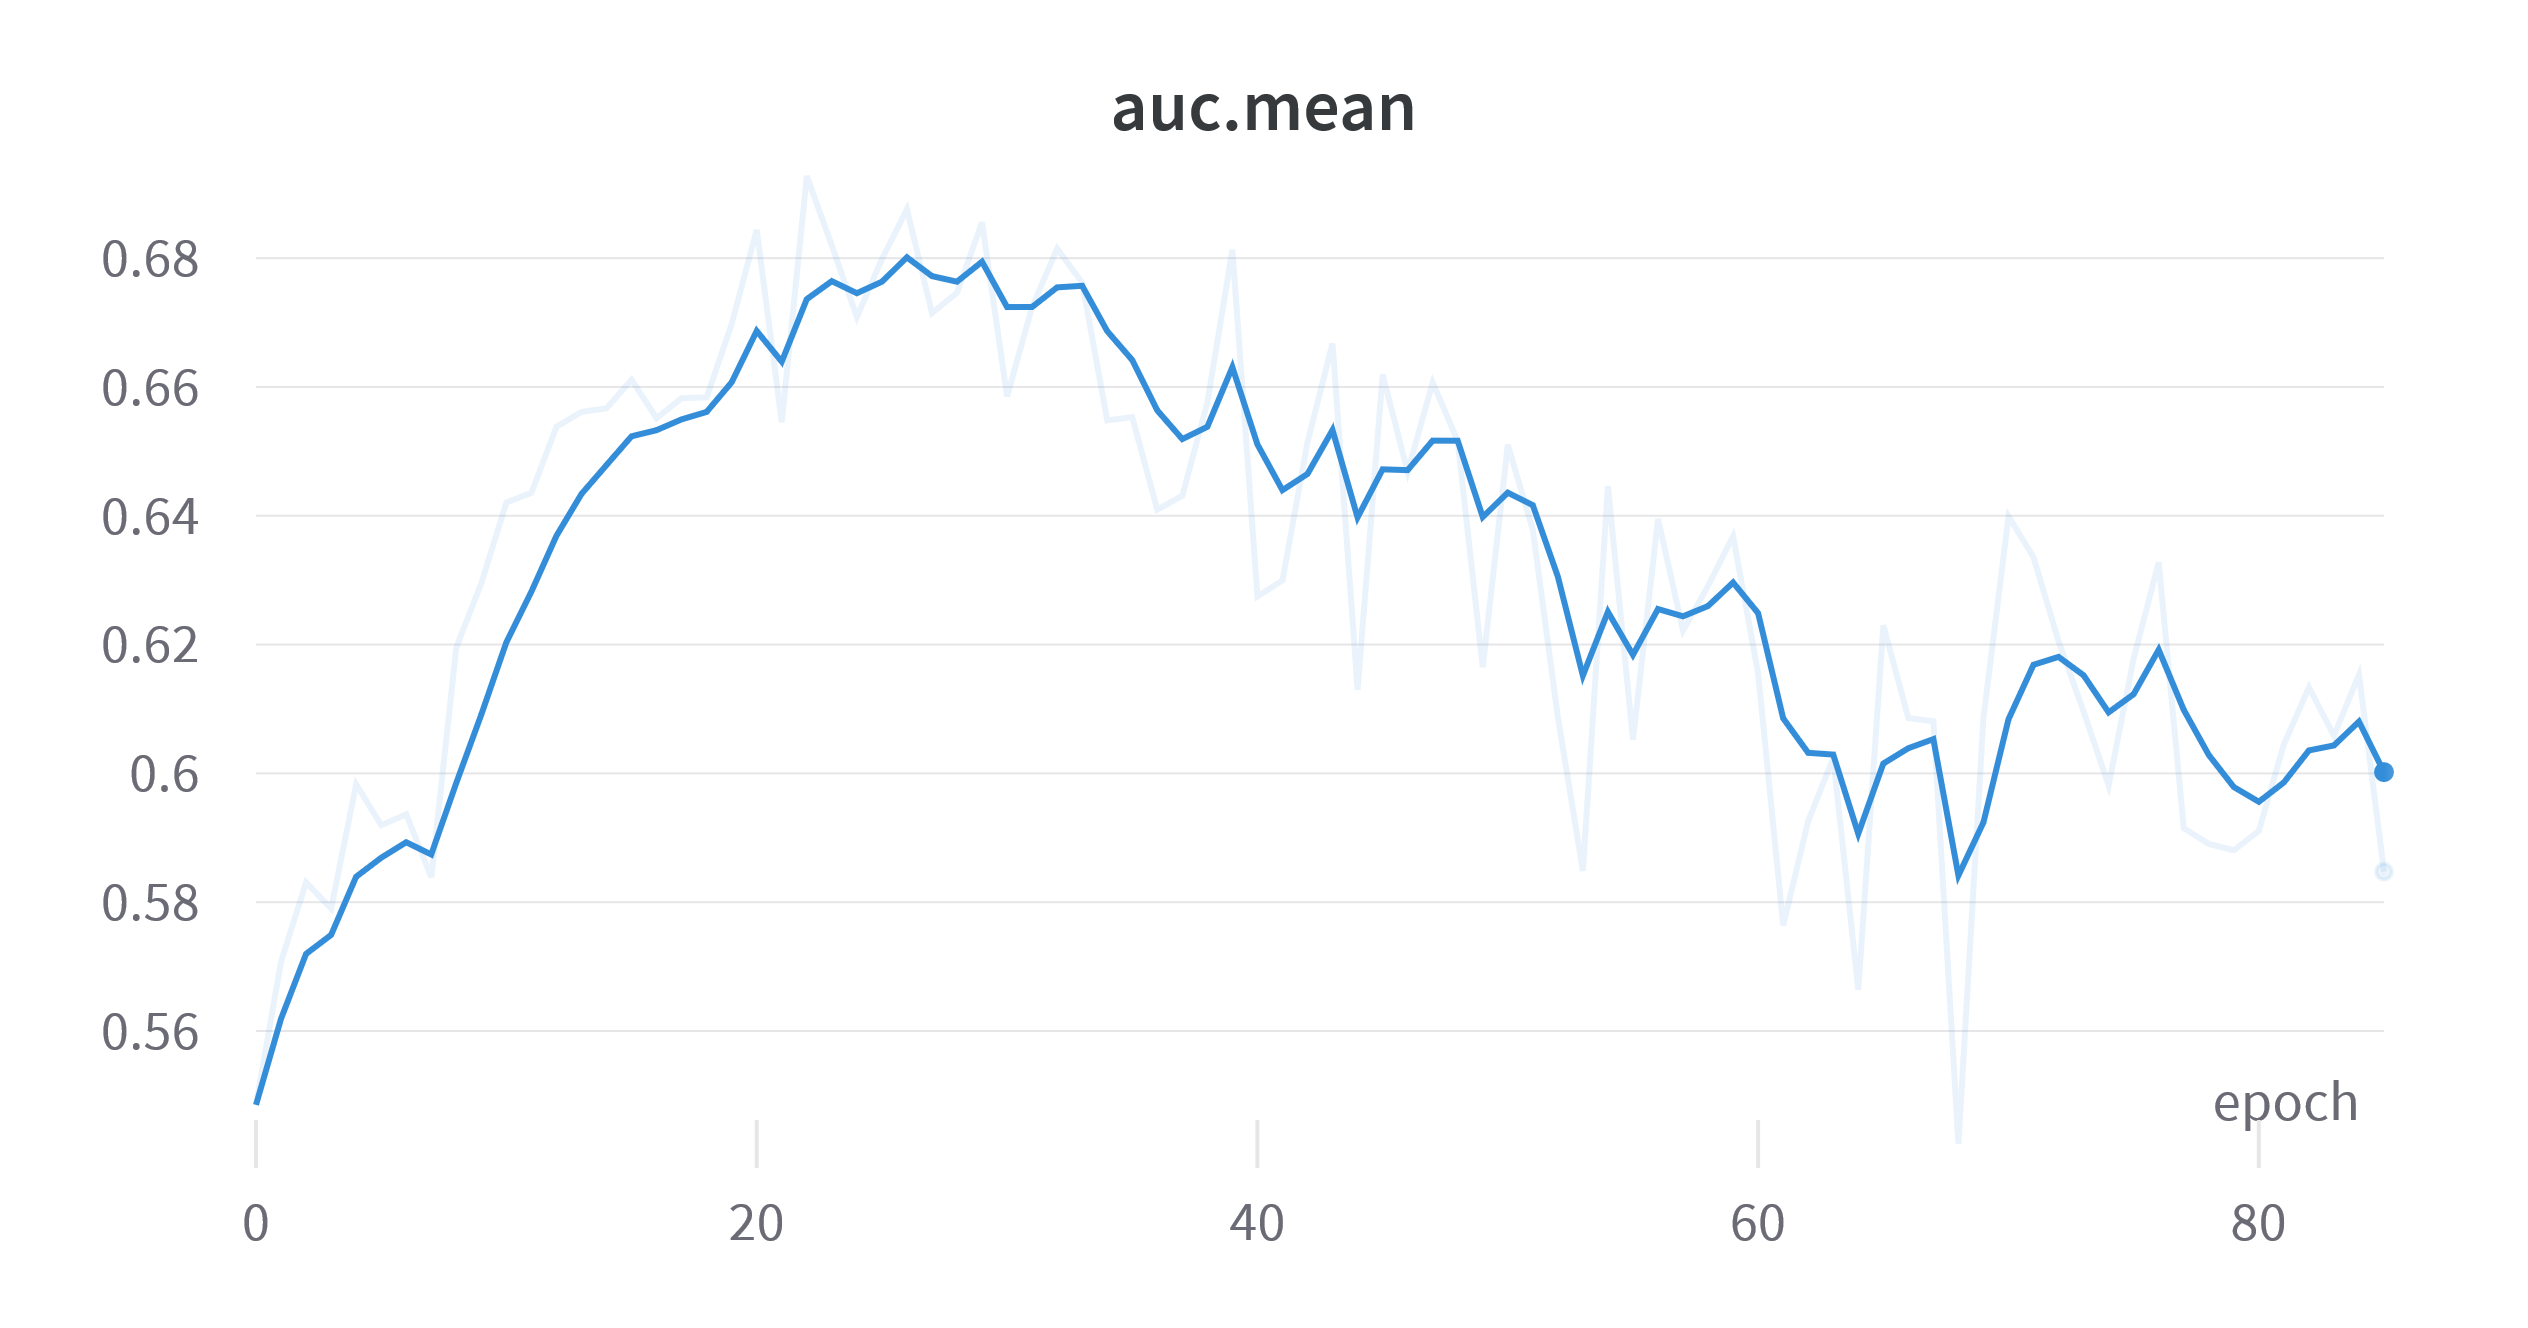
\includegraphics[width=\textwidth]{plots/chexpert_auc_3}
                     \caption{Validation loss}
                     \vspace{4ex}
                     \label{fig:chexpert_auc_3}
                 \end{subfigure}
                 \label{fig:chexpert_results3}
                 \caption{Metrics curves for our third attempt at reproducing the CheXpert baseline. The average values
                 include classes with no positive labels in the validation set. It should therefore only be used qualitatively. The curves are smoothed
                 out for an easier visualization.}

            \end{figure}
            \begin{table}[]
            \centering
            \begin{tabular}{llllll}
            \hline
            \multicolumn{1}{c}{Classes} &
               &
              \multicolumn{1}{c}{\begin{tabular}[c]{@{}c@{}}AUC\\ CheXpert\end{tabular}} &
              \multicolumn{1}{c}{\begin{tabular}[c]{@{}c@{}}F1-Score\\ (Radiologist's \\ estimation)\end{tabular}} &
              \multicolumn{1}{c}{\begin{tabular}[c]{@{}c@{}}AUC\\ (Ours)\end{tabular}} &
              \multicolumn{1}{c}{\begin{tabular}[c]{@{}c@{}}F1-Score\\ (Ours)\end{tabular}} \\ \hline
            Cardiomegaly     &  & 0.832 & 0.7  & 0.74 & 0.60  \\
            Pleural Effusion &  & 0.934 & 0.7  & 0.90 & 0.65  \\
            Pneumothorax     &  & N/A   & N/A  & 0.87 & 0.22  \\
            Lung Opacity     &  & N/A   & N/A  & 0.88 & 0.834 \\
            Atelectasis      &  & 0.858 & 0.68 & 0.67 & 0.47  \\
            Lung Lesion      &  & N/A   & N/A  & 0.26 & 0.67  \\
            Pneumonia        &  & N/A   & N/A  & 0.70 & 0     \\
            Consolidation    &  & 0.899 & 0.4  & 0.75 & 0.45  \\
            Edema            &  & 0.941 & 0.6  & 0.86 & 0.55  \\
            No Finding       &  & N/A   & N/A  & 0.89 & 0.93  \\ \hline
            \end{tabular}
            \end{table}
            To obtain these results, we used the following hyper-parameters :
            \begin{multicols}{2}

            \begin{itemize}
                \centering %TODO : correct layout ; verify all hyperparameters
                \item backbone : convnext small
                \item batch size : 64
                \item learning rate : 1e-4
                \item weight decay : 1e-2
                \item dropout : 0
                \item num samples per epoch : 50 000
                \item optimizer : AdamW
                \item scheduler : OneCycle
                \item patience : 20
                \item label smoothing : 0
                \item clip norm : 1
                \item epoch : 50
                \item channel : 3
                \item augment prob [ 1, 1, 0.5, 1, 1 ]
            \end{itemize}
            \end{multicols}
        \subsubsection{Lesson learned}
            % What did we learn from this experiment?
            The results of our last run was a bit of a deception. While we did manage to achieve a lower BCE loss than before,
            we did not manage to improve the AUC and F1-score significantly. While we cannot know for certain , a few factor more
            likely contributed to this. The first one is the three classes with low representation in the dataset. Since only randomly predicting
            a few true positive greatly increase the average AUC and F1-score without improving really the model's ability to predict the true positive,
            it biases our choice of model towards that one epoch which performed better in these unrepresentative categories.
            In future runs, we should either remove these classes from our metrics calculation or from our model's prediction. This is why from now we will exclude fractures
            and lung lesions as classes for our model.



            % The Cross entropy loss does not allow for a good comparison between the different models. We should use the AUC or the F1-score instead.
            We also see that the Cross-Entropy does not allow for a good comparison between the different models, as it does not correlate well with the AUC and F1-score.
            Ideally, a loss that allow to optimize more closely the AUC and F1-score would be better suited for this task. We will try and explore if such solution exists.
            % The patience mechanism should be based on the f1-score instead of the loss.
            Since our model's loss does not correlate well with the AUC and F1-score, we should use the F1-score as the metric to determine when to stop training. Our patience
            will therefore from now on be based on our F1-score instead of the loss.
            % The model with the positive weights is able to achieve a better AUC and F1-score.
            % The model with 3 channels is able to achieve a better AUC and F1-score.
            % The model with the convnext backbone is able to achieve a better AUC and F1-score.

            Finally, lowering the learning rate, in combination with the usual OneCycle scheduler allowed the model to reach a lower training and validation loss.


        \subsection{Reproducing the CheXpert competition's results}

            The CheXpert dataset was released as part of a competition, where the goal was to achieve the best possible performance on the hidden test set. The competition was won by a team from Stanford, who achieved a score of 0.91 on the hidden test set. The results of the competition are reported in the table~\ref{table:chexpert_competition_results}.
            The metric used was the ROC-AUC. We will therefore use the same metric to compare our results with theirs. However , we also implemented the
            F1-score (the harmonic mean of the precision and recall), which will make it easier to compare with the radiologist's performance
            in order to convince them to use our model.


        \subsubsection{DeepAUC~\cite{DeepAUC}}

            Attempting to reproduce the results of DeepAUC~\cite{DeepAUC} proved not to be possible. The snippet of code , provided by the author,
            did not reproduce the results as expected. No pretrained model was also given. Attempt to use their loss function with our dataset also proved
            to be unsuccessful. We therefore decided to not include their results in our comparison, and to not pursue this avenue.

        \subsubsection{Hierarchical Learning~\cite{hierarchical}}

            The hierarchical learning method~\cite{hierarchical} is a method that uses a hierarchy in between the different classes
            to more accurately predict them. Thansk to bayesian probabilities, we know that

            \begin{equation}
                P(A|B) = \frac{P(A \cap B)}{P(B)} = \frac{P(B|A) P(A)}{P(B)}
            \end{equation}

            If we use the parent class as B, with the child class as A, we can therefore redefine
            the probability of the child class such that

            \begin{equation}
                P(Child|parent) = \frac{P(Child \cap parent)}{P(parent)} \approx P(parent|Child) P(Child)
            \end{equation}

            We could use P(Parent) as the prior probability of the parent class, as defined by the preponderance in the dataset. However, as I base myself of~\cite{hierarchical}, I observe they did no such thing and I decided to not do it either. While this mean the probability given by the model might be based off an approximation,
            it also avoids having an additional bias in the model originating from the specific distribution of the training set. Further thought might however be given to this in order to evaluate the potential benefit of it.

            Since the classes we are interested in slightly differ from the ones used in~\cite{hierarchical},
            we will have to adapt the hierarchy. The hierarchy used in~\cite{hierarchical} is reported in the figure~\ref{fig:hierarchical_learning_hierarchy}. We will use the same hierarchy, but with our classes instead of theirs.


            They also used a pretraining phase, with only the case where the parent class is present. We will first try without this pretraining phase to see if it is necessary.



        \subsubsection{JFHealthcare - Probabilistic-CAM~\cite{jfhealthcare}}

            \begin{figure}[H]

                 \centering
                 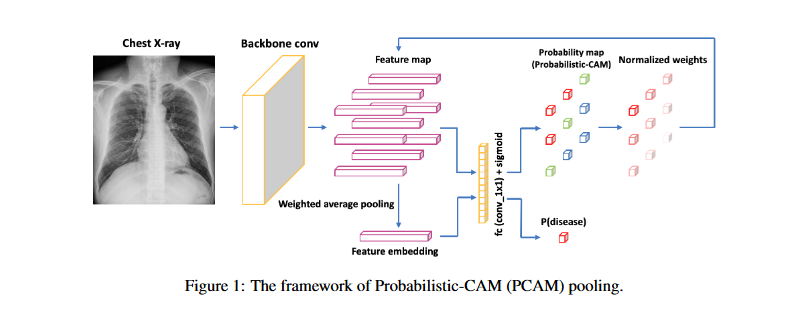
\includegraphics[width=0.8 \textwidth]{plots/jfhealthcare}
                 \caption{The figure 1 from~\cite{jfhealthcare}}
                 \label{fig:jfhealthcare_probabilistic_cam}

            \end{figure}

            The JFHealthcare team~\cite{jfhealthcare} used a probabilistic-CAM method to obtain their results.
            The method is based on the idea that the model should be able to predict the probability of a class being
            present in the image. The method is described in the figure~\ref{fig:jfhealthcare_probabilistic_cam}.

            They first start by proceeding as usual, applying a feature extraction backbone, followed by a 1x1 convolutionnal layer.
            They then apply a sigmoid activation function to the output of the fully connected layer, in order to obtain a probability between 0 and 1.

            These classes probability are then used as the probability of a disease being present in each of the feature maps. The feature maps are then
            weighted according to these probabilities using a weighted average pooling. This is then followed by a fully connected layer (with a sigmoid activation), which is used to output
            the final prediction.


            This adds two benefits . The first one is to enable a form of self-attention within the model which they have shown increase the accuracy of the model.
            But further than that, it also allows for a better understanding of the model's decision. Indeed, the weighted class activation maps offer a more accurate way to visualize the model's decision and potential object location
            within the image. This is especially useful for the radiologist, who might want to understand why the model made a certain decision.


        \subsection{Results on the CIUSSS dataset}


            Following the results obtained earlier on CheXpert, we then tried applying some of the same technique, but this time using a validation dataset from the CIUSSS data.
            For the training data, we tried to supplement the CIUSSS dataset with the CheXpert dataset, in order to increase the size of the dataset and improve the model's performance.




    \section{Explainability \& Visualization}

    %GradCam and improvements

    \section{Improvements and attempts}

    \subsection{Moving Average Labels}


    \section{Problem observed}

    A multitude of problems slowed down the development of the model. We will try to cover the most
    important ones here, and the lesson learned from them.


    \subsection{Normalizing the data}

        While the data was at first simply normalize by the mean and standard deviation of the ImageNet dataset.
        However, we realized this was not enough . This easily led to unstability in the training process, and we had to further
        normalize the input. The first attempt at this was with a min max normalization to rescale between 0 and 1, before applying the ImageNet's normalization
        .While this solved the issue, we did try to further improve the normalization by using the CLAHE algorithm. This algorithm is used to improve the contrast of the image, and is often used in medical imaging.

    \subsection{Verifying the data}
            The data was not as cleaned as we would have liked. While the CheXpert validation dataset was validated by a team of three radiologist, our data
            was simply annotated by a single radiologist's report, from which the labels were then automatically derived. This lead to a quite important source of error as radiologist's performance
            is estimated to be between 0.4 and 0.6~\cite{radiologist_performance}. This is a quite important source of error, which is compounded
            by the fact that the radiologist's report often contained many uncertainties that we had
            to quantify with an automated labeler. The problem's come that no radiologist was available to verify the work of the labeler, and we had to rely on our interpretation of
            the report to evaluate the performance of the rule-based labeler we developped.

            While it usually would simply be solved by manually annotating a few examples and compare the results accrosss the manually labeled dataset
            and the automatically labeled one, this was not possible in our case. Indeed, the nature of our medical dataset required an expert eye to verify the data,
            and even then, radiologists often disagree on the label of a given image. This is why when working on medical data, it is important to have a team of specialist available to support the project.


    \subsection{Drivers \& CUDA}

        Many times did we had issues with our drivers. This happened because we were updating the packages as we were developping the project, and because we were working on parallel on more than one project
        on the same machine. To rectify and avoid this, a simple solution is to use a virtual environment, which will allow us to have a clean environment for each project, and to avoid any conflict. Docker
        is a good solution to provide such virtual environment.

    \subsection{Multi-GPU training}

        To train on multiple GPU, I first used the DataParallel module from PyTorch. However, this module is deprecated, and I therefore chose to switch to the DistributedDataParallel module. This module is more efficient, but it is also more complicated to use.
        Just as to prove this point, it often break down, seemingly at random, and I had to restart the training process.

        While in and of itself it would only be annoying, the real problem is that the training would not simply stop, but would not converge, leading to
        wrong conclusion when trying to compare the results of the different models. It seems like the problem might arise from the synchronization of the
        gradient between the batches on each GPU. You see, compared to data parallel, the distributed data parallel instead of splitting the model between the GPUs, it splits the data between the GPUs.
        This means that the gradient are computed on each GPU, and then synchronized between the GPUs.

        This is a problem that I have not been able to solve, and I have not been able to find any solution to it online. I have therefore decided to switch back to the DataParallel module, which is less efficient, but at least it works.


    \subsection{Data augmentation}


        At first, I tried to implement a few technique of data augmentation of my own, as the torchvision library does not provide a lot of data augmentation technique.
        However, I quickly realized that the data augmentation technique I implemented were not as good as I wanted, being both not optimized enough and containing errors I would catch from time to time.

        Later, I found the Albumentations library~\cite{albumentations}, which is a library that provides a lot of data augmentation technique, and is very easy to use. I therefore decided to switch to this library, and it has proven to be a very good choice.
        It allowed me to quickly and easily test a few different data augmentations without worrying about potential errors in my implementation.

        However, it is not idiot-proof either. As I was working on the project, I later found a bug where my image input of format (C,H,W) was not being converted to (H,W,C) by the library, as it required, but was still processed, leading to disastrous images.

        To avoid this step, a jupyter notebook was then used to verify the output of our dataloader at different step in order to verify the integrity of the image
        throughout its pre-processing.

    \subsection{Unitary Tests}

            Based on the experience described above, I also decided to implement unitary testing in order to limit the errors
            that could be introduced in the code. The master branch of the git repository was also linked to these unitary tets such that
            any pull requests would first have to pass the tests before being merged into the branch. This is especially useful when working with a group,
            but even when working alone it is a good way to ensure that the code is working as intended and catch unintentional errors.


    \subsection{Unstability during training}

    \subsubsection{Automatic Mixed Precision (AMP)}

            To solve this problem, I tried to implement the automatic mixed precision (AMP) technique~\cite{automatic_mixed_precision}. This technique is a way to train a model in a lower precision, while still using a higher precision for the gradient computation.
            This is especially useful when training on a GPU, as it allows to reduce the memory usage, and therefore to train on larger batch size.

            However, this technique is not without its problems. Indeed, it is not always easy to implement, and it is not always compatible with all the libraries used.
            While this technique improved the training time vastly, it did lead to some unstability, with the gradient sometimes underflowing and becoming NaN.

            This is a problem that I have mostly solved by normalizing further the input vector but some underflowing might still occur. In these case, the training need to be done
            again as the model will be corrupted (Nan values in the weights).


    \subsubsection{Gradient's clipping}

        While we already experienced some unstability before, we mostly tried to solve it by normalizing the input.
        However, we still had some issues with the training process. To avoid overflowing gradients, we tried to use the gradient clipping technique \cite{gradient_clipping}.
        This technique is a way to limit the gradient to a certain value, in order to avoid them from exploding.

        By default, we set the maximum gradient norm to 1, but we also tried to set it to 2, and to 5. However, we found that the best results were obtained with a maximum gradient norm of 1.
        This also serves as a way of regularizing the model, as it forces the gradient to be small, and therefore forces the model to learn slowly.


    \section{Deploying the model}

        \subsection{Backend}

            The backend of the application is written in Python, using the Flask framework. The backend is responsible for the communication between the frontend and the model.
            It is also responsible for the preprocessing of the images, and for the prediction of the model.

            The backend is deployed on a server, and is accessible through an API.

        \subsection{Frontend}

            The frontend of the application is written with the Dash framework~\cite{dash}. This framework is a wrapper around the Flask framework, and allows to create a web application.

            This web application is accessible through a web browser, and allows the user to upload an image, and to get the prediction of the model. It also allow to use a few example
            preloaded in the server. This will allow us to easily display the capacity of the model, and to gather feedback from the user.

            Please give the appropriate credit to the authors of the template use to developped the web application.\footnote{It was developped by the Dash team and is available
            at \url{https://github.com/plotly/dash-sample-apps/tree/main/apps/dash-image-processing}}

            %Include images and description of the web application

        \subsection{Data Verification}
            %Unet
    \newpage
    % REFERENCES
    {
    \small

    \printbibliography
    }
\end{document}